    \documentclass[a4paper,12pt, twoside]{article}
    \usepackage[a4paper, left=2.5cm, right=2.5cm, top=2.5cm, bottom=2.5cm, bindingoffset=0.5cm]{geometry}
    \usepackage[utf8x]{inputenc}
    \usepackage{polski}
    \usepackage[polish]{babel}
    \usepackage{graphicx}
    \usepackage{indentfirst}
    \usepackage{float}
    \usepackage{caption}
    \usepackage{adjustbox}
    \usepackage{array}
    \usepackage{makecell}
    \usepackage{amsmath}
    \usepackage{enumitem}
    \usepackage{afterpage}
    \usepackage{subfig}
    \usepackage{hyperref}
    \usepackage{url}
    \usepackage{listings}
    \usepackage{xcolor}
    
    %New colors defined below
    \definecolor{codegreen}{rgb}{0,0.6,0}
    \definecolor{codegray}{rgb}{0.5,0.5,0.5}
    \definecolor{codepurple}{rgb}{0.58,0,0.82}
    \definecolor{backcolour}{rgb}{0.95,0.95,0.92}
    
    %Code listing style named "mystyle"
    \lstdefinestyle{mystyle}{
      backgroundcolor=\color{backcolour},
      commentstyle=\color{codegreen},
      keywordstyle=\color{magenta},
      numberstyle=\tiny\color{codegray},
      stringstyle=\color{codepurple},
      basicstyle=\ttfamily\footnotesize,
      breakatwhitespace=false,         
      breaklines=true,                 
      captionpos=b,                    
      keepspaces=true,                 
      numbers=left,                    
      numbersep=5pt,                  
      showspaces=false,                
      showstringspaces=false,
      showtabs=false,                  
      tabsize=2
    }
    
    \lstset{style=mystyle}
    
    %słowa nie są łamane
    \tolerance=1
    \emergencystretch=\maxdimen
    \hyphenpenalty=10000
    \hbadness=10000
    
    \renewcommand\thesection{\arabic{section}.}
    \renewcommand\thesubsection{\arabic{section}.\arabic{subsection}.}
    \renewcommand\thesubsubsection{\arabic{section}.\arabic{subsection}.\arabic{subsubsection}.}
    \renewcommand{\lstlistingname}{Algorytm}% Listing -> Algorytm
    \frenchspacing
    \setlength{\parindent}{.5cm}
    \makeatletter
    \setlength{\@fptop}{0pt}
    \makeatother
    \linespread{1.5}
    \begin{document}
    	\newpage
    	\thispagestyle{empty}
    	\begin{center}
    		
    		\begin{figure}
    			\centering
    			
\includegraphics[width=7cm]{images/polsl_logo.jpg}
    			\vspace{.5cm}
    		\end{figure}
    		
    		{\fontsize{17}{17}\selectfont
    			\textsc{Politechnika Śląska \\[.3cm]
    				Wydział Automatyki, Elektroniki i~Informatyki  \\[.3cm]
    				Kierunek Teleinformatyka  \\[1.5cm]}
    			\textbf{Projekt inżynierski \\[0.7cm]}}
    		
    		\Large
    		{Elektroniczna plakietka konfigurowana z~urządzenia mobilnego \\[3.5cm]}
    		\Large{\begin{flushleft}
    				Autor: Jakub Legutko\\
    				Kierujący pracą: dr inż. Grzegorz Dziwoki\\[0.3cm]
    		\end{flushleft}}
    		
    		\normalsize
    		\vfill Gliwice, styczeń 2020
    	\end{center}
    	\newpage
    % 	\leavevmode\thispagestyle{empty}\newpage
    	\newpage
    	\thispagestyle{empty}
    	\tableofcontents
    	\newpage
    % 	\leavevmode\thispagestyle{empty}\newpage
    	\newpage
    	\clearpage
    	\setcounter{page}{1}
    	
    	\section{Wstęp}
    	
    	\subsection{Wprowadzenie}
    	Zmiany klimatyczne są coraz bardziej widoczne na świecie. Wycinka drzew jest jednym z~głównych powodów wzrostu emisji gazów cieplarnianych \cite{clima_causes}. Ograniczenie jej wpłynęłoby pozytywnie na poziom dwutlenku węgla znajdującego się w~atmosferze, co przełoży się na poprawę klimatu. 
    	
    	Druk wizytówek oraz identyfikatorów pochłania w~skali globalnej znaczące ilości papieru, jak również tuszu ze względu na ich jednorazowe wykorzystanie w~większości przypadków. Z~tego powodu ważne jest zastosowanie alternatywnej metody. Gdyby wykorzystać urządzenie, które można użyć wielokrotnie poprzez zmianę wyświetlanych danych, wyeliminowany zostałby papier, a także toner, którego produkcja pochłania około 3.2 kilograma gazów cieplarnianych \cite{cartidge_production} na kartridż zawierający 200 gramów toneru. Kolejną rzeczą jest recykling, któremu trzeba poddać niepotrzebne już identyfikatory oraz zużyte do ich produkcji kartridże.
    	
    	Idealnym rozwiązaniem do budowy takiego urządzenia wydaje się być papier elektroniczny (ang. \textit{e-paper}). Wyświetlane na nim dane można modyfikować dowolną ilość razy, dzięki czemu może być używany wielokrotnie, nie powodując zużycia dodatkowych surowców przy każdym kolejnym wykorzystaniu. Ponadto po wyświetleniu dostarczonych danych, wyświetlacz nie pobiera żadnej energii i~może zostać odłączony od źródeł zasilania.

    	\subsection{Cel projektu}
    	Celem projektu inżynierskiego jest zaprojektowanie i~zbudowanie elektronicznej plakietki identyfikującej z~wykorzystaniem wyświetlacza typu e-papier, mogącej zastąpić klasyczne, papierowe identyfikatory lub wizytówki. Prezentowane dane są przygotowywane i~przesyłane przez urządzenie mobilne za pomocą napisanej aplikacji.

    	\subsection{Podstawowe założenia projektowe}
    	Przed przystąpieniem do wykonania projektu przyjęte zostały podane niżej założenia projektowe:
    	
    	\begin{flushleft} Założenia dla części sprzętowej:
    	\begin{itemize}
    		\item użycie wyświetlacza wykonanego w~technologii papieru elektronicznego;
    		\item bezprzewodowa transmisja danych z~urządzenia mobilnego na wyświetlacz plakietki;
    	\end{itemize}
    	
    	\vspace{.5cm}
    	Założenia dla części programowej:
    	\begin{itemize}
    		\item opracowanie aplikacji na urządzenia pracujące pod kontrolą systemu Android:
    		\begin{itemize}
    		    \item przechowywanie wpisów z~danymi do wyświetlania;
    		    \item przechowywanie wzorców układów wyświetlania danych;
    		    \item możliwość wyświetlania danych w~różnych miejscach na ekranie;
    		\end{itemize}
    		\item napisanie oprogramowania sterującego mikrokontrolerem, do którego podpięty jest wyświetlacz;
    		\item możliwość wyświetlania podstawowych danych osobowych (imię i~nazwisko, nazwa firmy, adres, numer telefonu, email);
    	\end{itemize}
    	\end{flushleft}
    	
    	\subsection{Opis projektu}
    	Wykonanie projektu było głównie natury programowej. Napisano aplikację na urządzenia mobilne umożliwiającą wprowadzanie, przechowywanie i~przesyłanie danych do mikrokontrolera. Układy połączone są szeregowo. Koniecznym było dostosowanie przesyłanych danych do struktury, którą można przesłać połączeniem szeregowym. W~mikrokontrolerze z~kolei, dane te muszą zostać odebrane i~odróżnione od siebie. W~urządzeniu mobilnym dane zostają kodowane i~przesłane do mikrokontrolera, gdzie są dekodowane do postaci umożliwiającej ich wyświetlenie.
    	
    	Część fizyczna polegała na połączeniu ze sobą modułu wyświetlacza z~modułem mikrokontrolera i~zapewnienia im zasilania. 
	
    	\begin{flushleft}
    	Wykonanie projektu przebiegało w~kilku etapach:
    	\begin{itemize}
    	    \item konstrukcja części sprzętowej;
    	    \item napisanie programu dla mikrokontrolera do sterowania modułem plakietki elektronicznej;
    	    \item napisanie aplikacji dla urządzenia mobilnego;
    	    \item przeprowadzenie testów urządzeń i~aplikacji;
    	    \item wdrożenie rozwiązań zauważonych w~trakcie testów błędów;
    	\end{itemize}
    	\end{flushleft}
 
        \newpage
    	\section{Wykorzystane narzędzia}
    	W trakcie pracy nad projektem użyto narzędzi dostępnych w~ramach licencji zezwalających na korzystanie z~nich bez opłat, nawet w~projektach komercyjnych. Do wykonania projektu użyto następujących narzędzi.
    	
    	\subsection{Android}
    	Android Studio zostało wykorzystane do napisania aplikacji na urządzenia mobilne. Jest to oficjalne zintegrowane środowisko programistyczne \textit{(ang. integrated development environment)} \cite{ide} do produkcji aplikacji na system Android, bazowane na IntelliJ IDEA.
    	
    	\begin{figure}[H]
    	    \centering
    		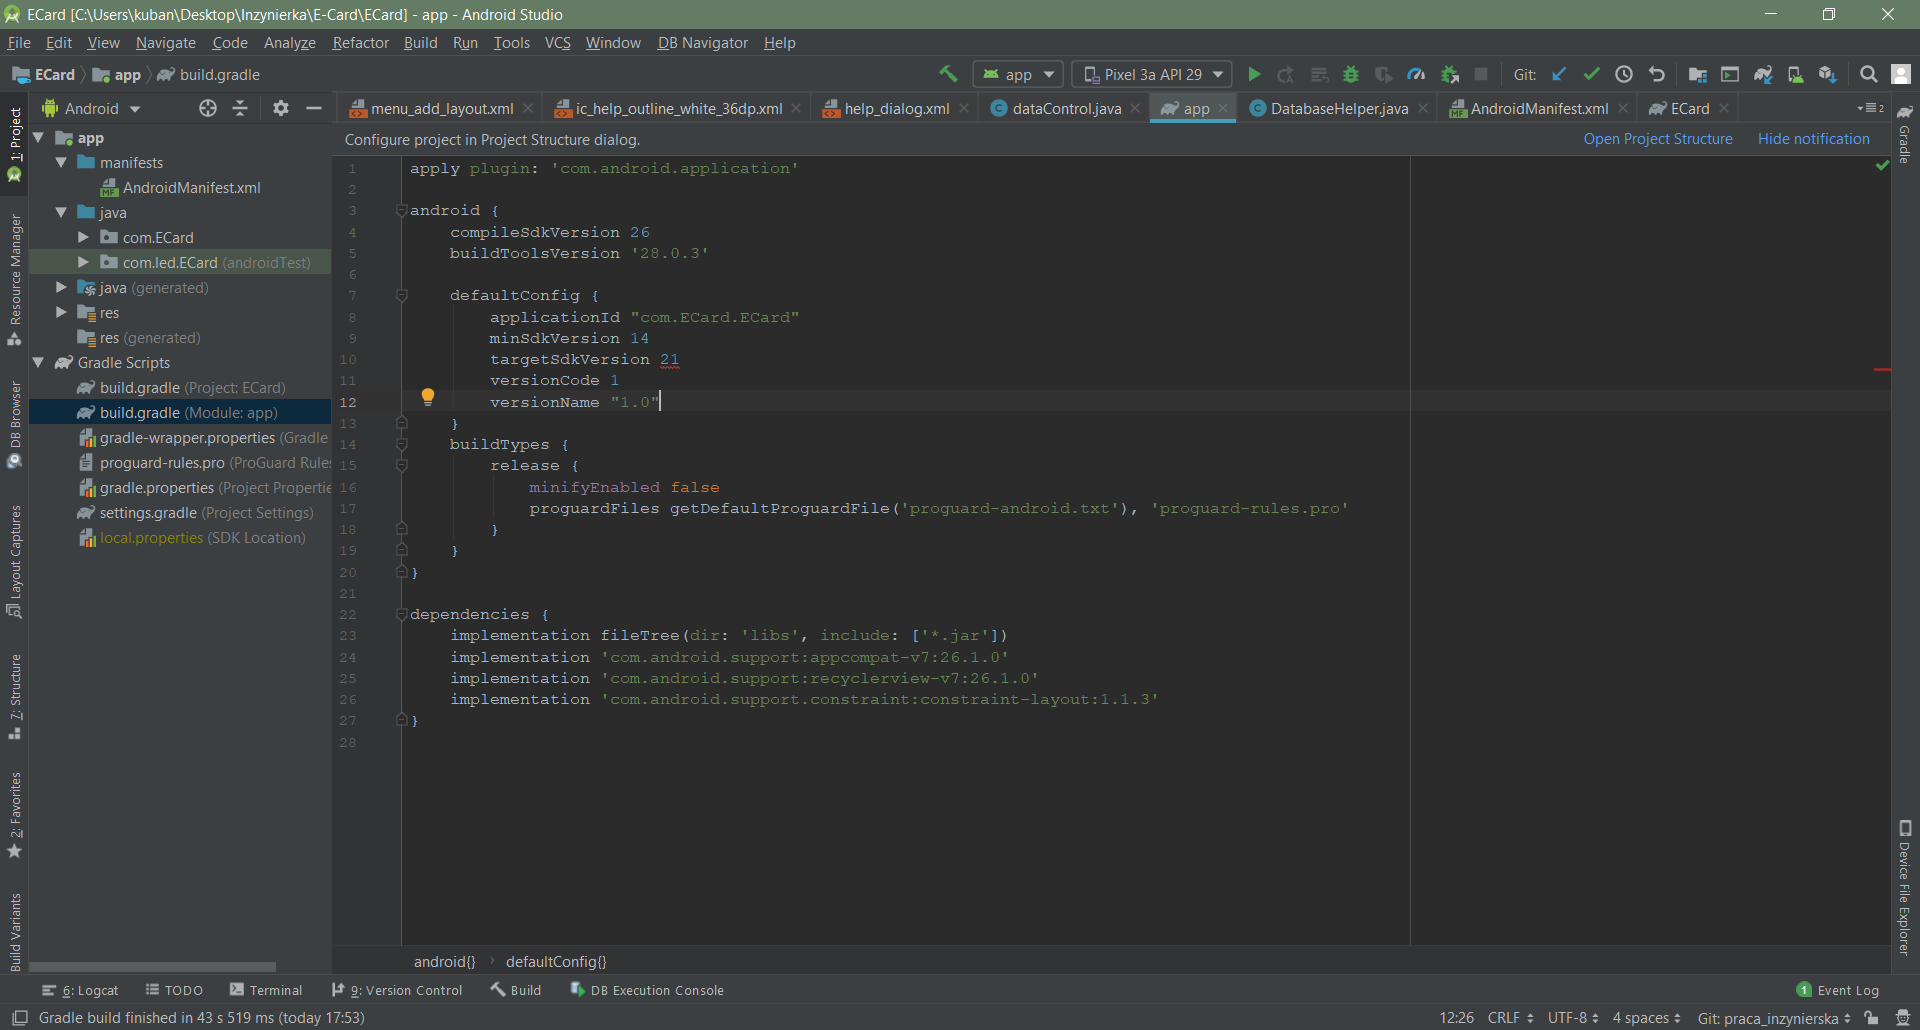
\includegraphics[width=1\textwidth]{images/rys4_android.png}
    		\caption{Widok Android Studio}
            \label{fig:androidstudio}
    	\end{figure}
     	
        Podczas realizacji projektu najczęściej wykorzystywaną funkcją, obecną w~Android Studio było podpowiadanie kodu wykonywane przez wbudowane w~środowisko szablony kodu \textit{(ang. live templates)}. Korzystanie z~szablonów daje możliwość skrócenia zapisu często pojawiających się części kodu do wpisania jednego słowa i~wybrania jego szablonu do wykonania. Na przykład wpisując w~edytorze słowo \textit{Toast}, który jest nazwą wykorzystanego szablonu, a następnie przejście po interaktywnej liście do odpowiedniej zmiennej i~zatwierdzeniu jej, spowoduje pokazanie jej zawartości. 
    
    \begin{lstlisting}[language=C++, caption=Zawartość szablonu Toast]
Toast.makeText(this, "", Toast.LENGTH_SHORT).show();\end{lstlisting}
    
        Kolejnym narzędziem zintegrowanym ze środowiskiem jest linter \cite{lint}. \textit{Lint} jest narzędziem analizującym kod źródłowy i~wykrywającym błędy składni i~struktury kodu źródłowego bez konieczności kompilacji lub uruchamiania aplikacji.
    
        Przy testowaniu aplikacji korzystano również z~wbudowanego w~Android Studio emulatora. Pozwoliło to przetestować działanie aplikacji na urządzeniach posiadających różne wersje systemu i~różne fizyczne rozmiary. 

    	Aplikacja mobilna została napisana w~języku Java. Jest to oparty na klasach, obiektowy język programowania. W~programowaniu dla Androida wykorzystuje się przygotowane dla niego SDK\textit{ (z ang. Software development kit)}\cite{sdk}.
    	
    	Aplikacja składa się z~aktywności, które posiadają swój cykl życia, przedstawiony na rysunku numer \ref{fig:lifecycle}. Metoda onCreate jest metodą uruchamianą jako pierwsza. W~niej wykonywane są funkcjonalności napisane dla aktywności.
    
    	\begin{figure}[H]
    	        \centering
    			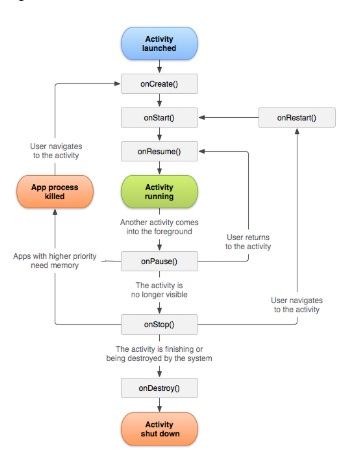
\includegraphics[width=8cm]{images/rys6_androidlifecycle.png}
    			\caption{Uproszczony ilustracja cyklu życia aktywności \cite{lifecycle}}
                \label{fig:lifecycle}
    	\end{figure}
    	
    	Widoki aplikacji budowane są w~wielu różnych plikach XML oraz klasach aktywności, gdzie istnieje możliwość tworzenia elementów programowo.
    	
    	\subsection{Arduino}
    	Arduino IDE jest wieloplatformowym zintegrowanym środowiskiem deweloperskim napisanym w~języku C oraz C++. Oparty jest na wolnej licencji GNU GPL v2.0. W~projekcie inżynierskim został wykorzystany do napisania i~zaprogramowania modułu mikrokontrolera.
    	
    	Programy pisane są w~językach C oraz C++ używających specjalnych struktur kodowania. W~języku tym zostało napisane również oprogramowanie mikrokontrolera. Udostępnionych do wykorzystania jest wiele bibliotek obsługujących szeroką gamę czujników, serw czy wyświetlaczy. Jedną z~takich bibliotek, która została wykorzystana w~projekcie jest biblioteka \textit{GxEPD} \cite{gxepd}. Biblioteka ta umożliwia obsługę wyświetlacza e-papieru. Dokładniej została opisana jest w~punkcie \ref{GxEPD}
    	
    	\begin{figure}[H]
    			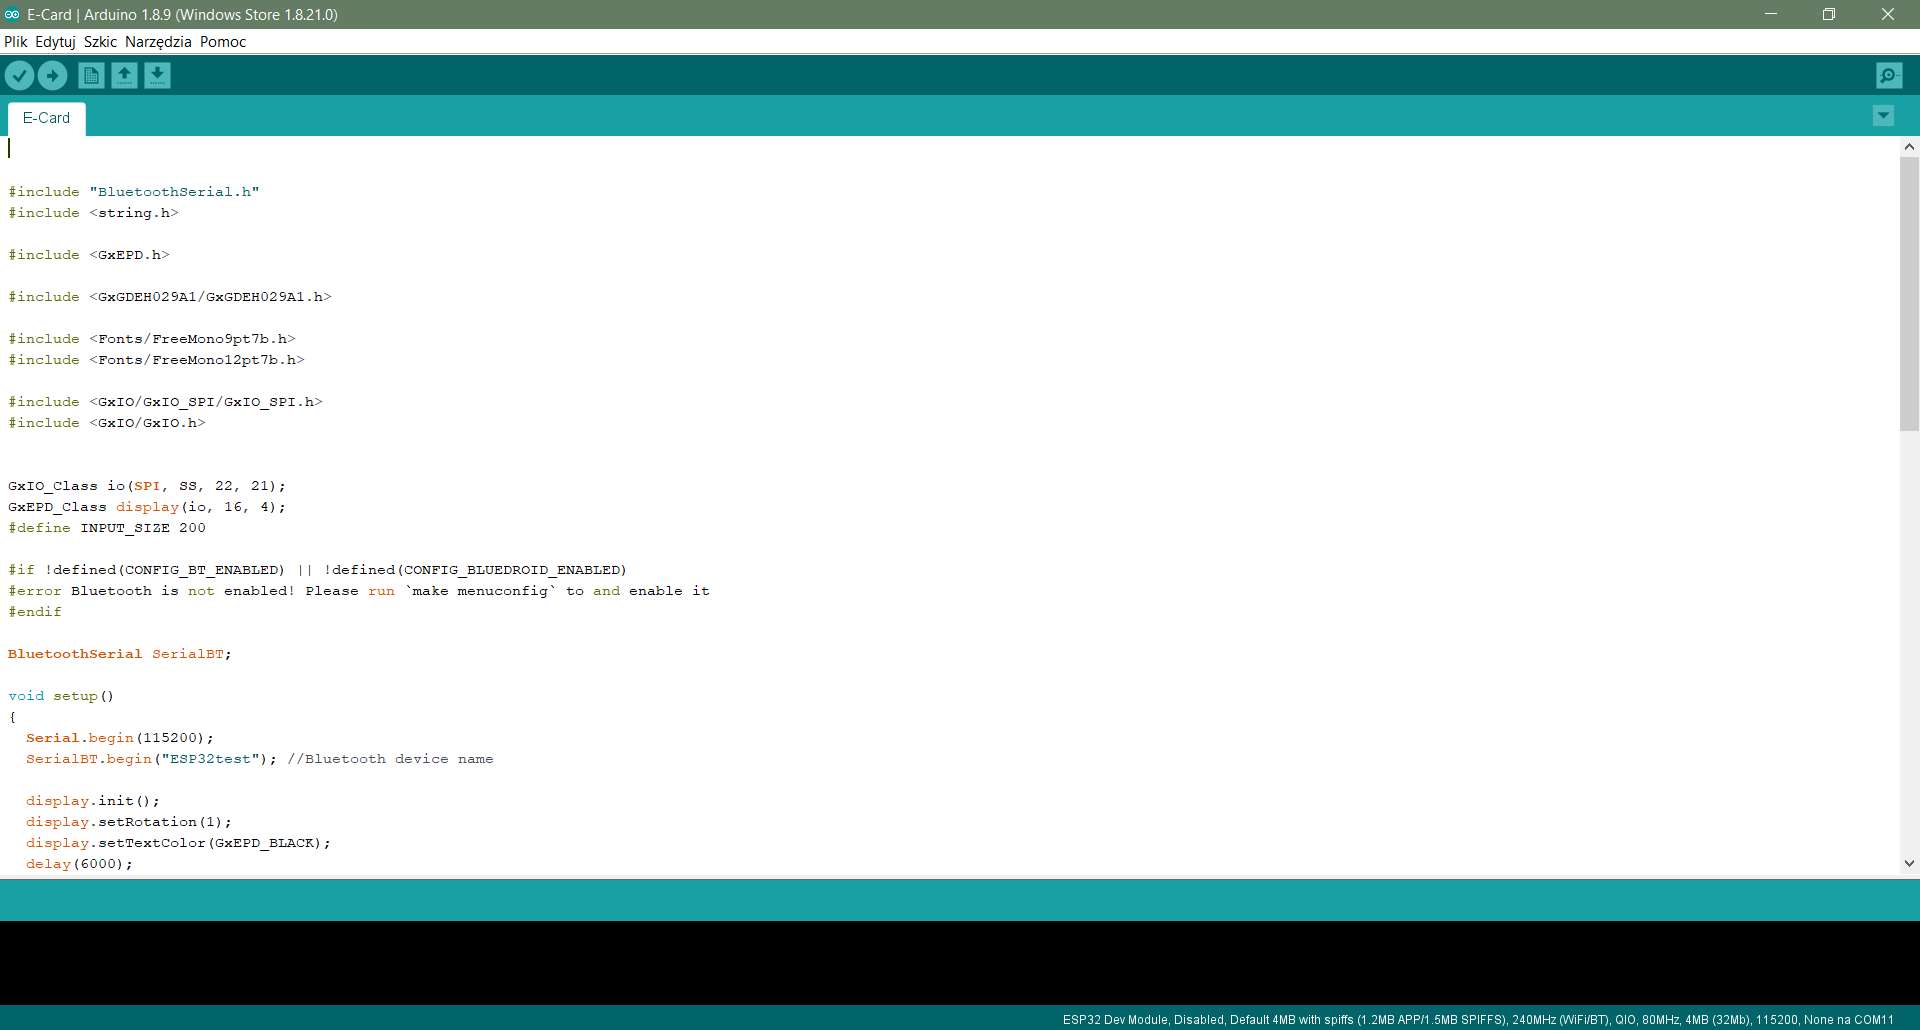
\includegraphics[width=1\textwidth]{images/rys3_arduino.png}
    			\caption{Widok Arduino IDE}
                \label{fig:arduinoide}
    	\end{figure}
    	
    	\subsection{SQLite}
    	SQLite to relacyjna baza danych dostępna na licencji \textit{public domain}\cite{publicdomain}, zostałą zaprojektowana w~2000 roku przez Richarda Hippa. Jest najczęściej używanym silnikiem baz danych na świecie. Występuje we wszystkich telefonach mobilnych oraz na większości komputerów. 
    	
    	Użycie SQLite w~projekcie zapewniło szybką i~intuicyjną budowę relacyjnej bazy danych. W~Androidzie dostępna jest klasa implementująca metody obsługi bazy SQLite. Baza odpowiada za przechowywanie wpisów danych do wyświetlania oraz układów wyświetlania danych. 
    	
    	\subsection{GxEPD}\label{GxEPD}
    	GxEPD jest biblioteką wykorzystywaną w~obsłudze wyświetlacza papieru elektronicznego. Dostępna jest na licencji GNU \textit{(ang. GENERAL PUBLIC LICENSE V3)}. Opiera się na stworzonej przez firmę Adafruit bibliotece Adafruit GFX dostępnej na licencji BSD \textit{(ang. Berkeley Software Distribution Licenses)} używanej do obsługi graficznych wyświetlaczy.
    	
    	GxEPD dziedziczy z~biblioteki Adafruit GFX, jednak jest ona przystosowana do działania z~wyświetlaczami papieru elektronicznego. Informacje wyświetlane na ekranie są buforowane i~przesyłane partiami. Takie rozwiązanie jest wykorzystane aby każdy obsługiwany przez bibliotekę procesor mógł wyświetlać dane. Nawet jeśli procesor posiada wystarczającą ilość pamięci RAM, dane są buforowane. Dane zostaną wyświetlone po odświeżeniu ekranu. Biblioteka posiada metody obsługujące pełne oraz częściowe odświeżanie ekranu. Przy wykorzystaniu odświeżania częściowego mamy znacznie mniejszy czas odświeżania w~porównaniu do odświeżenia całego ekranu.
    	
        Wykorzystane w~projekcie czcionki pochodzą z~biblioteki Adafruit GFX. Czcionki są w~formacie bitmapy, każdy znak zapisany jest w~bitach o~długości zależnej od jego wielkości. Glify reprezentowane są przez pięć wartości, dzięki którym wiadomo jakie dane opisują pojedynczy glif. Są nimi \textit{index,  Width, Height, xAdv, dX, dY}. Index informuje o~miejscu rozpoczęcia danych w~bitmapie dla danego glifu. Width oraz Height są to szerokość i~wysokość danego glifu. xAdvance informuje ile miejsca należy pozostawić pomiędzy znakami, pomaga zachować czytelność tekstu. dX jest odległością od początku układu do początku znaku w~osi odciętych. dY jest odległością od linii bazowej do początku glifu w~osi rzędnych. dX i~dY używane są w~celu wyznaczenia pozycji dla glifu. Dzięki nim można rozróżnić '-' oraz '\_', które w~postaci bitowej mogłyby być takie same. W~projekcie użyto dwóch rozmiarów czcionki FreeMono dostępnej w~ramach GNU FreeFont. Czcionka w~rozmiarze 9pt zajmuje mniej więcej 1516 bajtów, druga o~rozmiarze 12pt zajmuje około 2132 bajtów.
        
        Pobieranie znaków następuje poprzez wywołanie kodu ASCII odpowiedniego znaku z~pliku zawierającego czcionkę. Każda czcionka posiada strukturę definiującą początkowy i~końcowy znak ASCII dostępny w~czcionce oraz wskaźniki do bitmapy i~tablicy glifów.
        
        GxEPD oferuje prosty sposób wyświetlania znaków na ekranie wyświetlacza. Można korzystać z~metod \textit{print()} oraz \textit{println()} do przesyłania danych, w~taki sam sposób jak przesyła się dane do portu seryjnego. Następnie biblioteka zajmuje się pobieraniem odpowiednich znaków z~czcionki i~narysowaniem ich na wyświetlaczu piksel po pikselu. 
        
        \newpage
    	\section{Opis i~specyfikacja urządzenia}
    	Elektroniczna plakietka konfigurowana z~urządzenia mobilnego składa się z~dwóch części. Urządzenia mobilnego z~zainstalowanym oprogramowaniem napisanym do obsługi tego projektu oraz urządzenia będącego fizyczną częścią projektu, składającego się z~mikrokontrolera oraz wyświetlacza w~technologii elektronicznego papieru.
    
        W~rozdziale przedstawiono ogólny schemat projektu i~wybrane do jego wykonania podzespoły. Opisana została idea działania oraz algorytm, według którego działa program mikrokontrolera.
        
        \subsection{Opis części fizycznej projektu}
        \begin{figure}[H]
    	        \centering
    			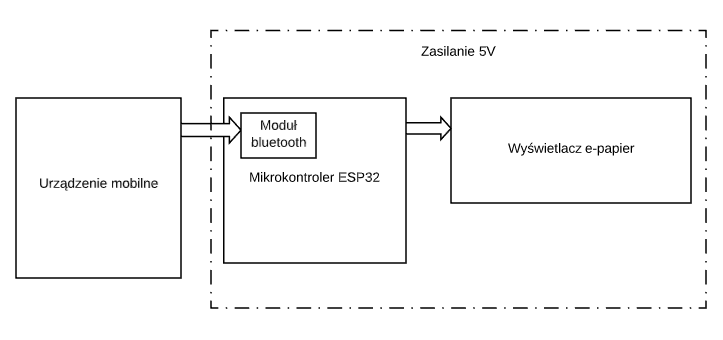
\includegraphics[width=12cm]{images/rys_7schemat_blokowy.png}
    			\caption{Schemat blokowy projektu}
                \label{fig:block}
    	\end{figure}
        Urządzenie imitujące papierowy identyfikator zostało zaprojektowane z~wykorzystaniem mikrokontrolera ESP32 firmy Espressif. Mikrokontroler posiada wbudowany moduł \textit{Bluetooth}, który jest wykorzystywany do nawiązywania połączenia z~urządzeniem mobilnym oraz transmisji danych pomiędzy nimi. Do wyświetlania przesyłanych danych używany jest wyświetlacz papieru elektronicznego firmy Waveshare.
        
        \begin{flushleft}
        \textbf{Opis poszczególnych bloków układu}
        \end{flushleft}
        \begin{enumerate}
            \item \textbf{Urządzenie mobilne} wykorzystane w~obsłudze wyświetlacza papieru elektronicznego musi posiadać wersję systemu Android OS w~wersji co najmniej 4.0.3. Niektóre z~wykorzystanych funkcji systemu Android, jak na przykład animowane przechodzenie pomiędzy aktywnościami, mogą wymagać do działania nowszej wersji systemu, jednak nie jest to konieczne.
            Kolejnym wymogiem korzystania z~pełnej funkcjonalności projektu, jest obecność modułu Bluetooth w~urządzeniu mobilnym. Bez jego obecności niemożliwe staje się przesłanie danych do mikrokontrolera, a zarazem wyświetlenie ich na papierze elektronicznym.
        
    	    \item \textbf{Mikrokontrolerem}, użytym w~projekcie jest 32-bitowy ESP32 firmy Espressif. Do wykonania projektu posłużono się modułem ESP32-DevKitC. Posiada on wbudowany port Micro-USB do zasilania i~programowania urządzenia oraz możliwość współpracy ze środowiskiem programistycznym Arduino. Moduł posiada 4MB pamięci flash\cite{flash}. Do dyspozycji użytkownika oddane jest jednak tylko 1.25MB z~dostępnej pamięci. Oprogramowanie napisane do wykonania projektu wykorzystuje niecałe 0.9MB pamięci mikrokontrolera, co pozostawia miejsce na dalsze rozwijanie projektu. ESP32 posiada zintegrowany w~chipie moduł Bluetooth wykorzystywany do transmisji danych pomiędzy urządzeniem mobilnym a mikrokontrolerem.
    
    
            \item \textbf{Wyświetlacz papieru elektronicznego} to 2.9-calowy ekran firmy Waveshare. Może pracować w~dwóch napięciach roboczych 3.3V oraz 5V. Zasilany jest przez wyjście 3.3V dostępne w~ESP32. Jest w~stanie wyświetlać dane w~dwóch kolorach (białym i~czarnym) z~czasem potrzebnym do pełnego odświeżenia wyświetlacza równym w~przybliżeniu 2 sekundy \cite{waveshare}. Każdy piksel zbudowany jest z~wielu cząstek (białych i~czarnych) osadzonych w~przezroczystym płynie. Wyświetlanie znaków odbywa się poprzez zmianę ładunku elektrycznego dla każdego piksela ekranu. Zależnie od znaku ładunku elektrycznego przyciągane są białe lub czarne cząstki, powodując zmianę koloru piksela. E-papier nie potrzebuje zasilania do zachowania stanu pikseli.\newpage
            
            Schemat ideowego połączenia wyświetlaczem z~modułem mikrokontrolera:
            \begin{figure}[H]
    	        \centering
    			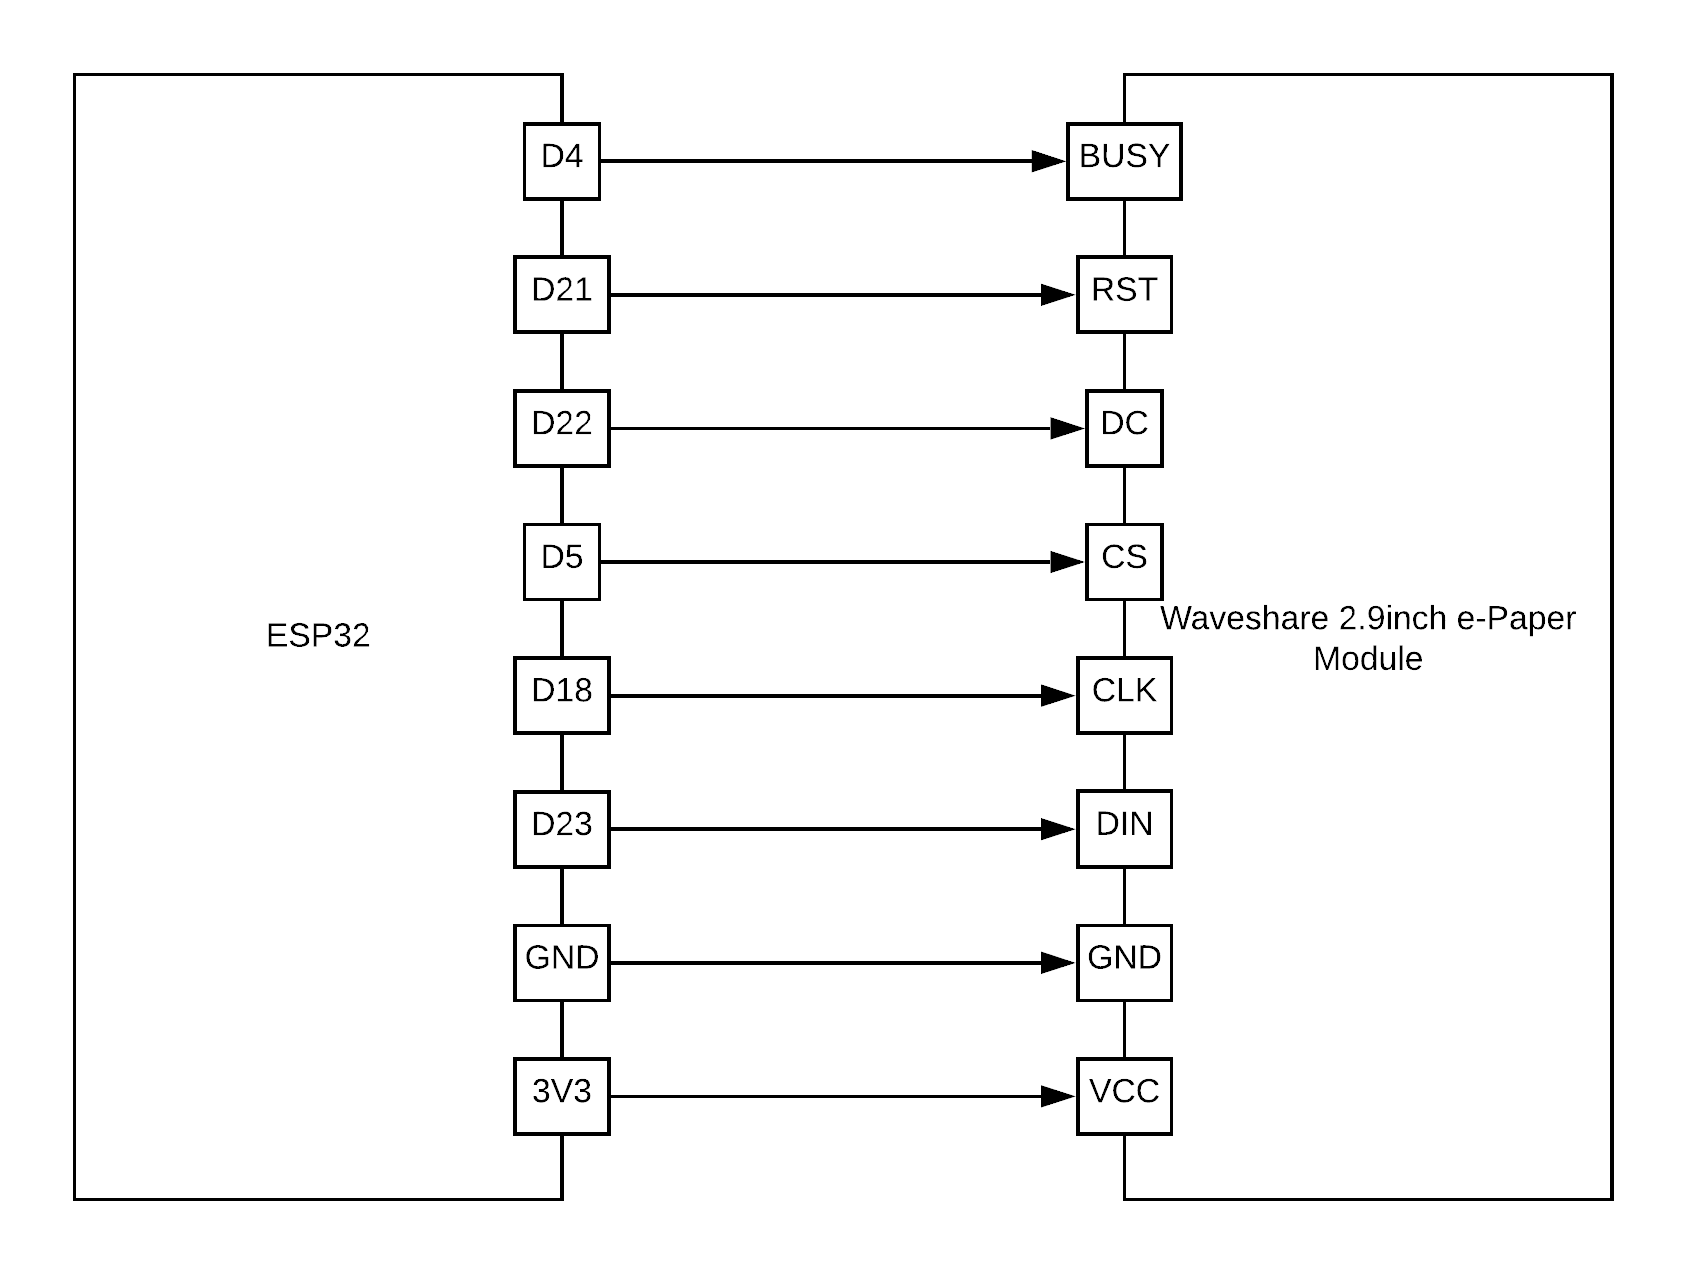
\includegraphics[width=12cm]{images/schemat_polaczenia_mikro_z_wyswietlaczem.png}
    			\caption{Schemat ideowego połączenia wyświetlaczem z~modułem mikrokontrolera}
                \label{fig:polecznie_mikro_z_epapierem}
    	    \end{figure}
        
            Wyprowadzenia  wyświetlacza papieru elektronicznego: 
            \begin{itemize}
                \item \textbf{VCC, GND} — dostarczanie zasilania wyświetlaczowi;
                \item \textbf{DIN, CLK, CS} — wyprowadzenia wykorzystywane przez interfejs szeregowy SPI. CLK jest linią zegara. Przez DIN dane przesyłane są z~mikrokontrolera (mastera) do wyświetlacza (slave). CS używany jest do wyboru aktywnego urządzenia (stan niski), w~naszym projekcie podłączone mamy tylko jedno urządzenie więc jest ono zawsze aktywne;
                \item \textbf{DC} — wybór przesyłania danych lub komend do wyświetlacza. Stan wysoki dla danych, stan niski dla komend;
                \item \textbf{RST} — zewnętrzny reset, aktywowany stanem niskim;
                \item \textbf{BUSY}  — linia wyjściowa wyświetlacza wykorzystywana do przesyłania informacji do mikrokontrolera o~stanie zajętości wyświetlacza. Przy stanie aktywnym (aktywność przy niskim stanie) wyświetlacz nie będzie reagował na komendy przesłane przez mikrokontroler; 
            \end{itemize}
        \end{enumerate}
        
        \subsection{Opis części programowej mikrokontrolera}
    	Program sterujący działaniem mikrokontrolera został napisany w~zintegrowanym środowisku programistycznym Arduino IDE. Program jest kompilowany, a następnie przesyłany do mikrokontrolera za pomocą wbudowanego w~moduł programatora.

        Oprogramowanie można podzielić na dwie części. Jedną odpowiedzialną za konfigurację mikrokontrolera oraz drugą, w~której jest wykonywana nieskończona pętla \textit{(loop)}, gdzie opisane jest działanie programu.
        
        W~pierwszej części ustalane są wyprowadzenia mikrokontrolera, z~których będzie korzystał program do połączenia z~wyświetlaczem. Sprawdzane jest również czy moduł Bluetooth jest uruchomiony. 
        \begin{lstlisting}[language=C++, caption=Konfiguracja wykorzystanych modułów]
//ustawienie wyprowadzen uzytych do polaczenia z~wyswietlaczem
GxIO_Class io(SPI, SS, 22, 21);
GxEPD_Class display(io, 16, 4);

#if !defined(CONFIG_BT_ENABLED) || !defined(CONFIG_BLUEDROID_ENABLED)
#error Bluetooth is not enabled! Please run `make menuconfig` to and enable it
#endif
\end{lstlisting}

        Następnie tworzone są obiekty odpowiadające za transmisję szeregową poprzez moduł Bluetooth i~rozpoczyna się rozgłaszanie nazwy urządzenia. Inicjowane jest również połączenie z~wyświetlaczem.
        \begin{lstlisting}[language=C++, caption=Konfiguracja wykorzystanych modułów]
Serial.begin(115200);
SerialBT.begin("ESP32test"); //nazwa urzadzenia bluetooth
display.init();
\end{lstlisting}

    	Druga część programu jest wykonywana w~nieskończonej pętli. Schemat działania pętli przedstawiony został na rysunku numer \ref{fig:petlamikrokontrolera}. Tutaj tworzone są wykorzystywane w~programie zmienne wraz z~przypisanymi im wartościami startowym.
    	
    	Głównym zadaniem pętli jest nasłuchiwanie portu szeregowego modułu Bluetooth. Otrzymane na porcie RX dane, zapisywane są do zmiennej. Dane wejściowe składają się z~parametrów służących do obsługi wyświetlania i~elementów do wyświetlenia na ekranie. Każdy element oddzielony jest od kolejnego specjalnym znakiem. Dane te przetwarzane są do postaci, którą można wysłać i~wyświetlić na wyświetlaczu papieru elektronicznego. 
    	
    	Do rozdzielania otrzymanych danych z~portu szeregowego Bluetooth na słowa wykorzystywana jest funkcja dostępna w~języku C jaką jest \textit{strtok} \cite{strtok}. \label{petladekod}Ogranicznikiem po wykryciu którego, następuje podział danych przesłanych z~urządzenia mobilnego jest \textit{';'}. Dane kopiowane są do tablicy z~wykorzystaniem funkcji \textit{strcpy} \cite{strcpy}, która jest dostępna w~języku C, w~klasie string.h. 
    \begin{lstlisting}[language=C++, label={lst:petlaprzepisujaca}, caption=Działanie pętli przepisującej otrzymane dane do tablicy]
char *ptr = strtok(input, ";");
while (ptr != NULL) {
  strcpy(ch_arr[i], ptr);
  ptr = strtok(NULL, ";");
  i++;
}\end{lstlisting}
    
        Po przepisaniu wszystkich informacji do tabeli program zaczyna procedure wysyłania danych do wyświetlacza. Wykorzystana w~programie tablica jest dwuwymiarowa. Jej wymiarem jest [21][27]. Wymiary zostały wybrane ze względu na ilość przesyłanych słów,  oraz maksymalną możliwą długość słowa mieszczącą się w~jednej linii wyświetlacza. Program do poprawnego wyświetlenia wszystkich otrzymanych elementów potrzebuje dwadzieścia jeden słów. Pierwsze przesyłane słowo jest wykorzystywane do ustalenia rotacji ekranu. Dla każdego z~wyświetlanych elementów, którymi są imię i~nazwisko, nazwa firmy, adres, email i~numer telefonu, przesyłane są po 4 słowa:
        \begin{itemize}
            \item wielkość czcionki;
            \item współrzędna kursora X;
            \item współrzędna kursora Y;
            \item informacja do prezentacji na ekranie;
        \end{itemize}
    
    	Informacja musi posiadać wszystkie wymienione wyżej parametry, aby została wyświetlona.
    	
    	Na rysunku numer \ref{fig:petlamikrokontrolera}. zaprezentowany został schemat blokowy działania programu mikrokontrolera ESP32. Przedstawiono w~nim kroki wykonywane przed wejściem do pętli oraz jej działanie.
    	\begin{figure}[H]
    	        \centering
    			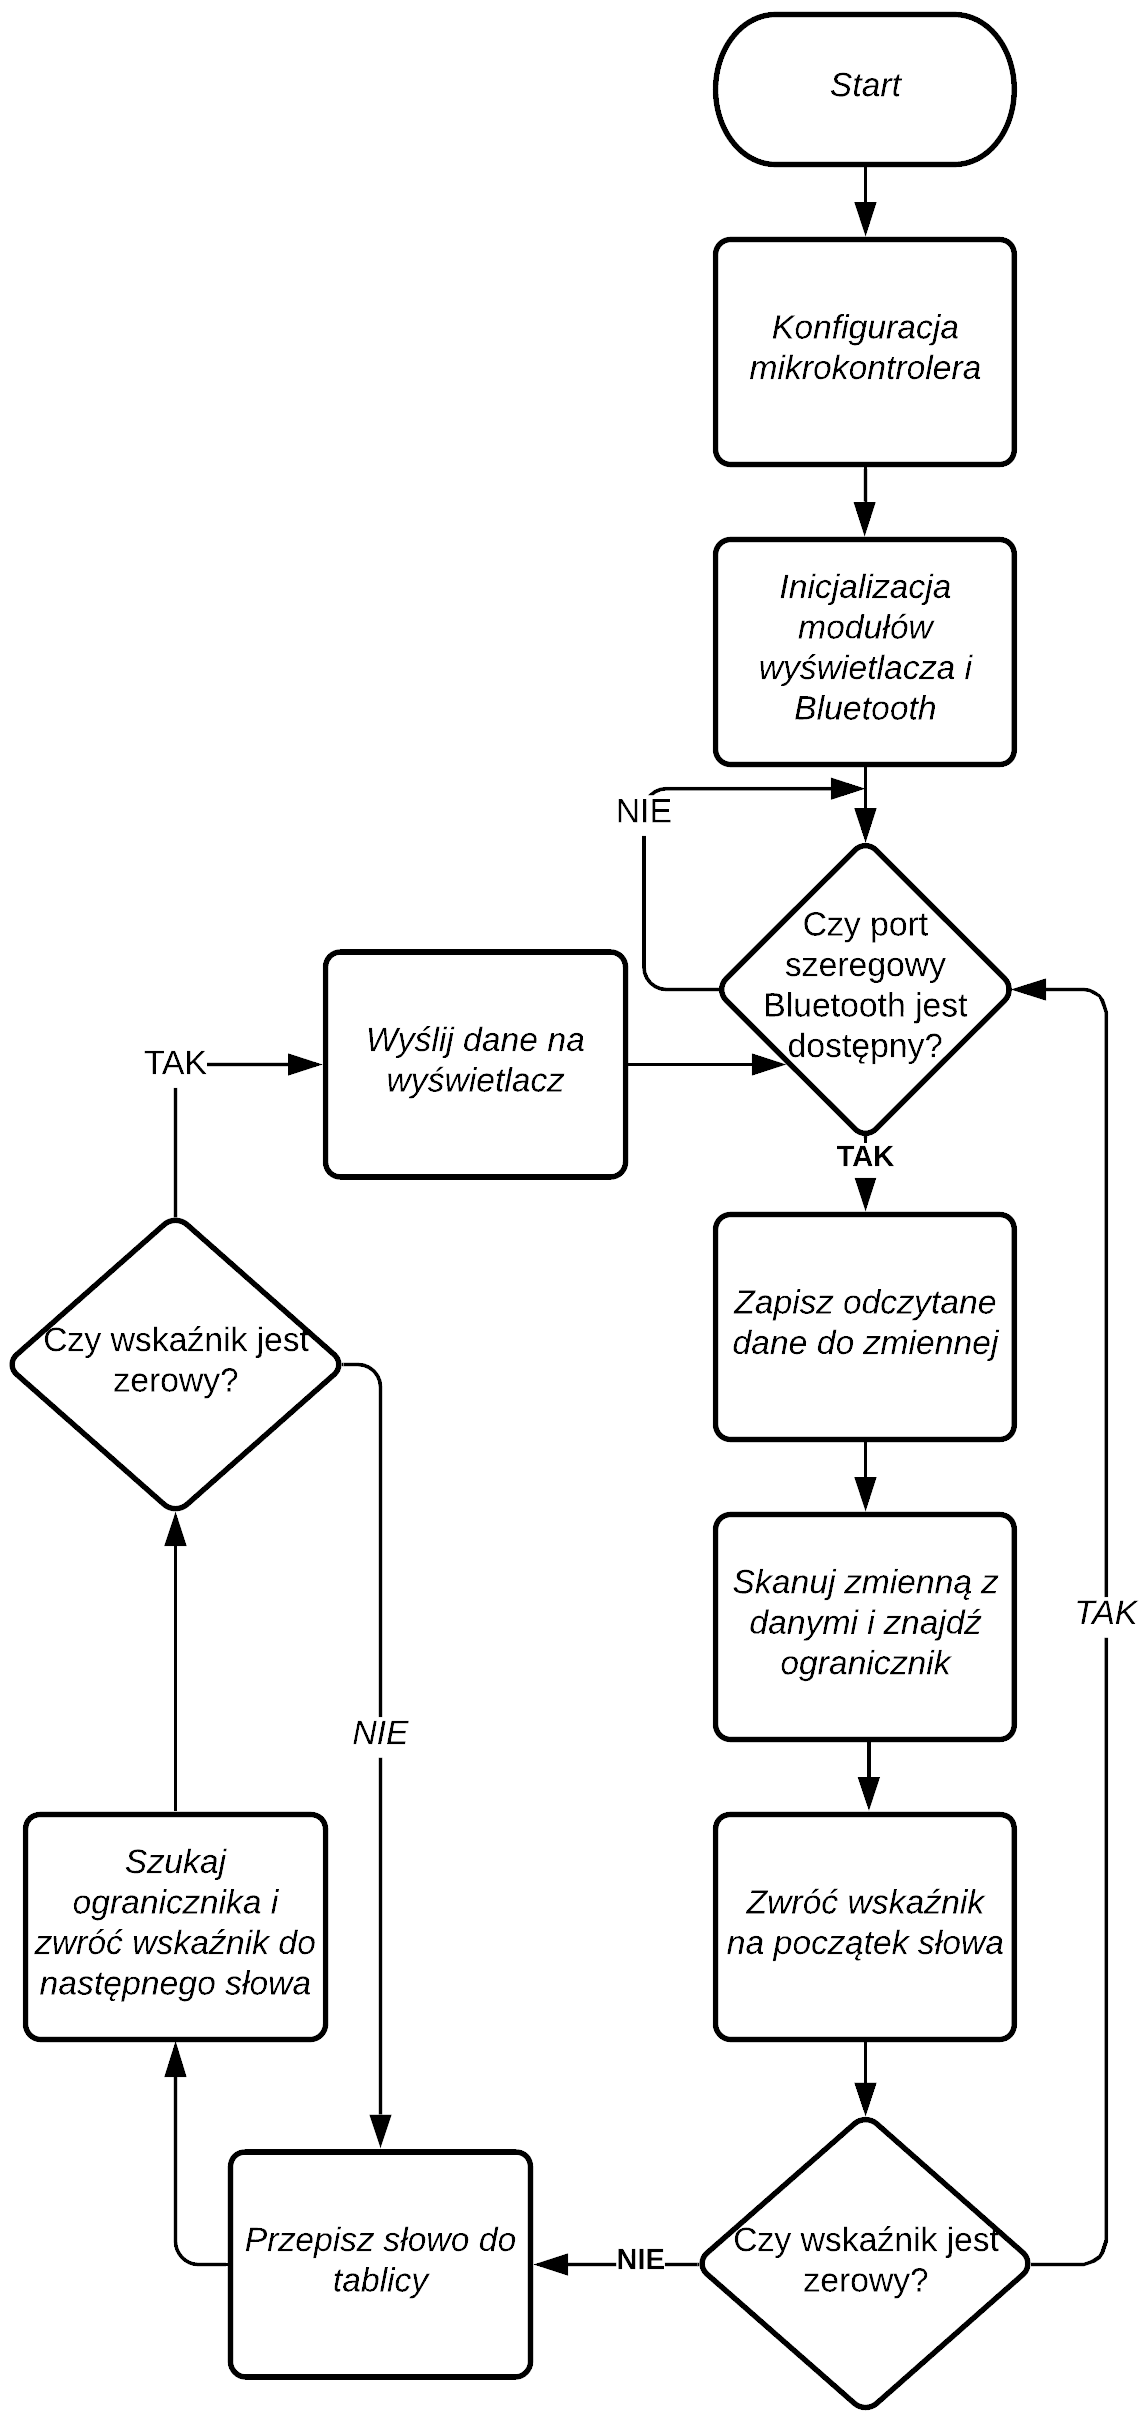
\includegraphics[width=9cm]{images/schemat_petli_mikrokontrolera.png}
    			\caption{Schemat blokowy działania programu mikrokontrolera}
                \label{fig:petlamikrokontrolera}
    	\end{figure}
    	
    	\section{Opis aplikacji}
    	Aplikacja na urządzenie mobilne została napisana dla systemu mobilnego Android w~środowisku Android Studio firmy Google. Środowisko to dostosowane jest do budowy aplikacji na system Android. Aplikację napisano w~języku Java z~obsługą minimalnej wersji API poziomu 15.
    	
    	Program zaprojektowano zgodnie ze wzorcem programowania obiektowego \textit{(Object Oriented Programming)}\cite{oop}, w~którym kod podzielony jest na części, które są łatwiejsze w~utrzymaniu i~konserwacji. Każda część jest samodzielna w~swojej funkcjonalności, zarazem możliwe jest wykorzystanie jej przez inne programy działające w~aplikacji. Wszystkie części działają wspólnie, tworząc całość aplikacji. Części te nazywane są obiektami. 
    	
    	Aplikacja posiada pięć aktywności odpowiadających za różne funkcjonalności. Do przechowywania danych użyto relacyjnej bazy danych SQLite. W~aplikacji można przechowywać zapisane dane do wyświetlenia na wyświetlaczu, jak również przygotowane i~zapisane układy wyświetlania.
    	\newpage
    	\subsection{Podział na aktywności}
    	\label{podzialnaaktywnosci}
    	Aplikacja składa się z~pięciu aktywności.
    	\begin{enumerate}
    	   \item \textbf{Devices} — jest aktywnością startową aplikacji. Głównym zadaniem \textit{Device list} jest prezentowanie na liście  sparowanych urządzeń Bluetooth.
    	   \begin{figure}[H]
    	    \centering
    		    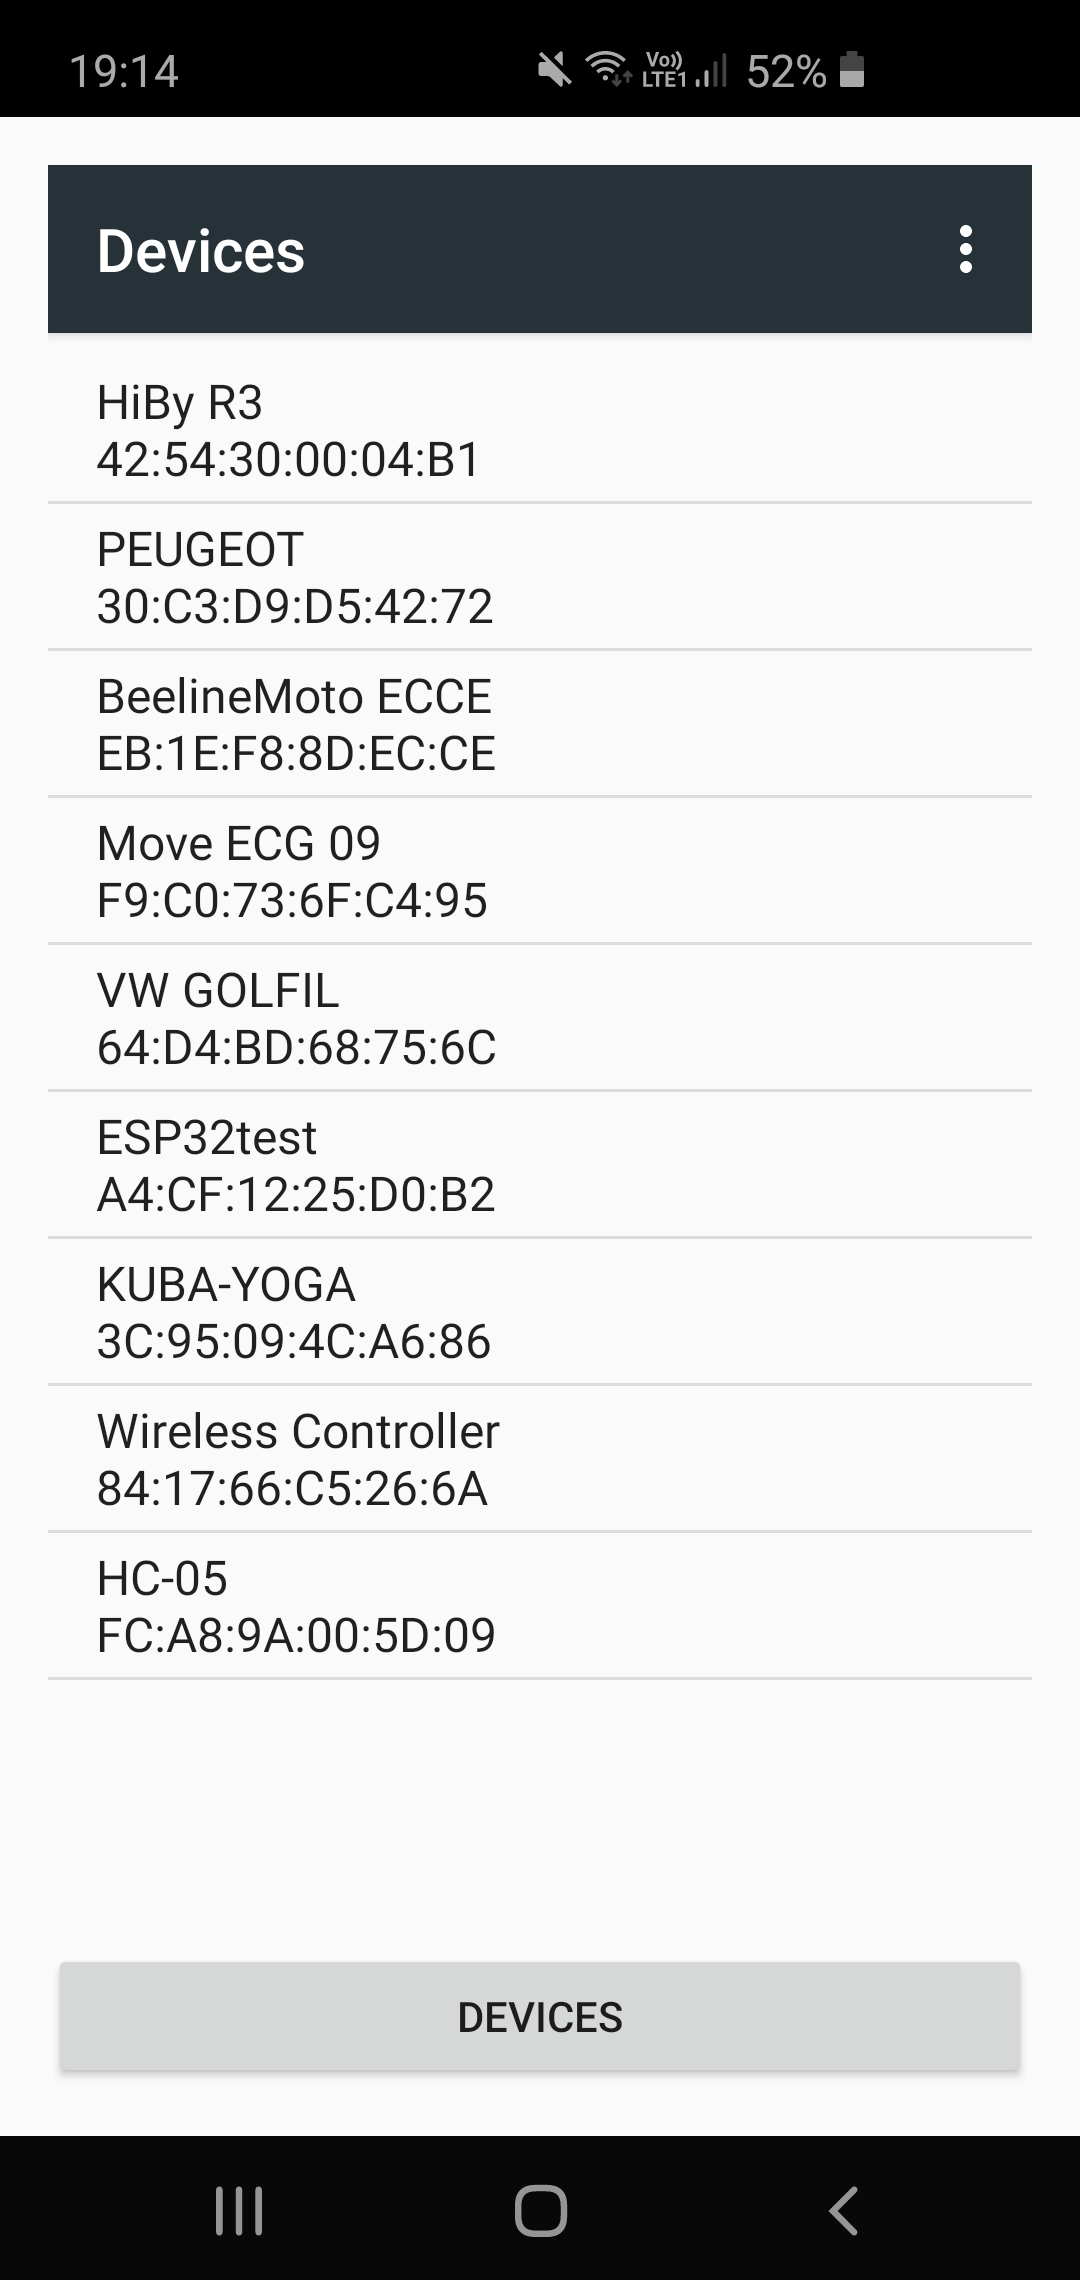
\includegraphics[width=5cm]{images/view_deviceList.jpg}
    			\caption{ Ekran wyświetlający listę sparowanych urządzeń}
                \label{fig:btdevices}
    	   \end{figure}
    	   Po utworzeniu aktywności sprawdzane jest czy urządzenie posiada moduł Bluetooth i~czy jest on włączony. Po spełnieniu tych warunków wyświetlane są sparowane z~urządzeniem mobilnym urządzenia Bluetooth. Po wybraniu urządzenia elektronicznej plakietki pobierany jest jego adres Bluetooth \textit{(ang. Bluetooth Device Address)}\cite{bdaddr} i~otwarta zostaje aktywność obsługi danych. Aktywność posiada rozwijane menu, z~którego można przejść do aktywności listy układów danych lub aktywności obsługi układów.
    	   \item \textbf{Data control} — najważniejsza aktywność całej aplikacji. Umieszczone są w~niej spinner, z~którego wybierany jest układ wyświetlania oraz pola edycji danych nazwiska, nazwy firmy, adresu, email i numeru telefonu. Posiada trzy przyciski sterujące funkcjonalnościami aktywności. Umieszczone jest w~niej również rozwijalne menu służące do przełączania aktywności.
    	   \begin{figure}[H]
    	        \centering
    	        \begin{minipage}{.5\textwidth}
    	            \centering
    	            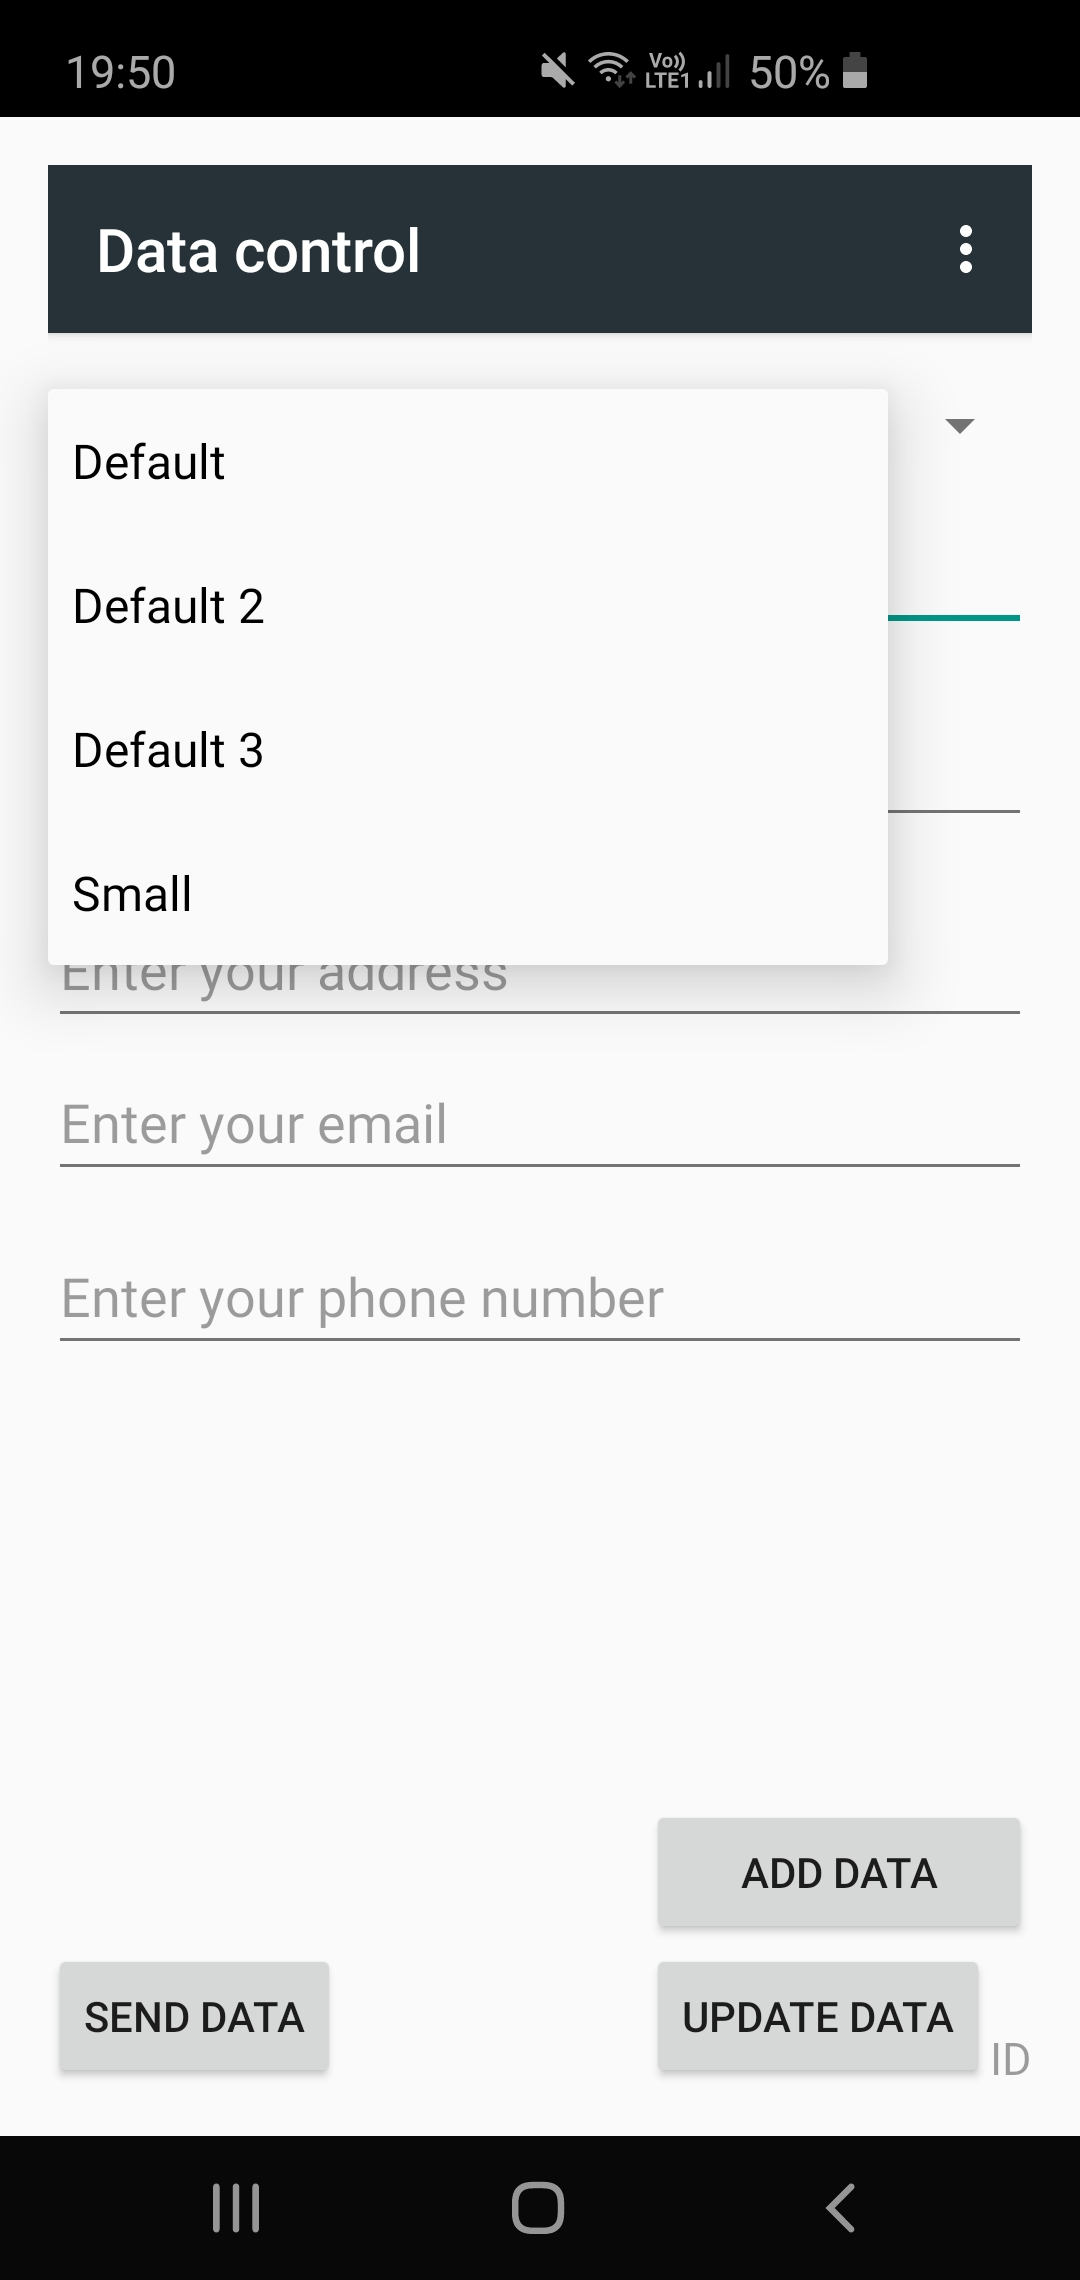
\includegraphics[width=5cm]{images/view_dataControl.jpg}
    	            \captionof{figure}{Ekran sterowania \newline danymi z~rozwiniętym spinnerem}
                    \label{fig:dataControl}
                \end{minipage}%
                \begin{minipage}{.5\textwidth}
                    \centering
    	            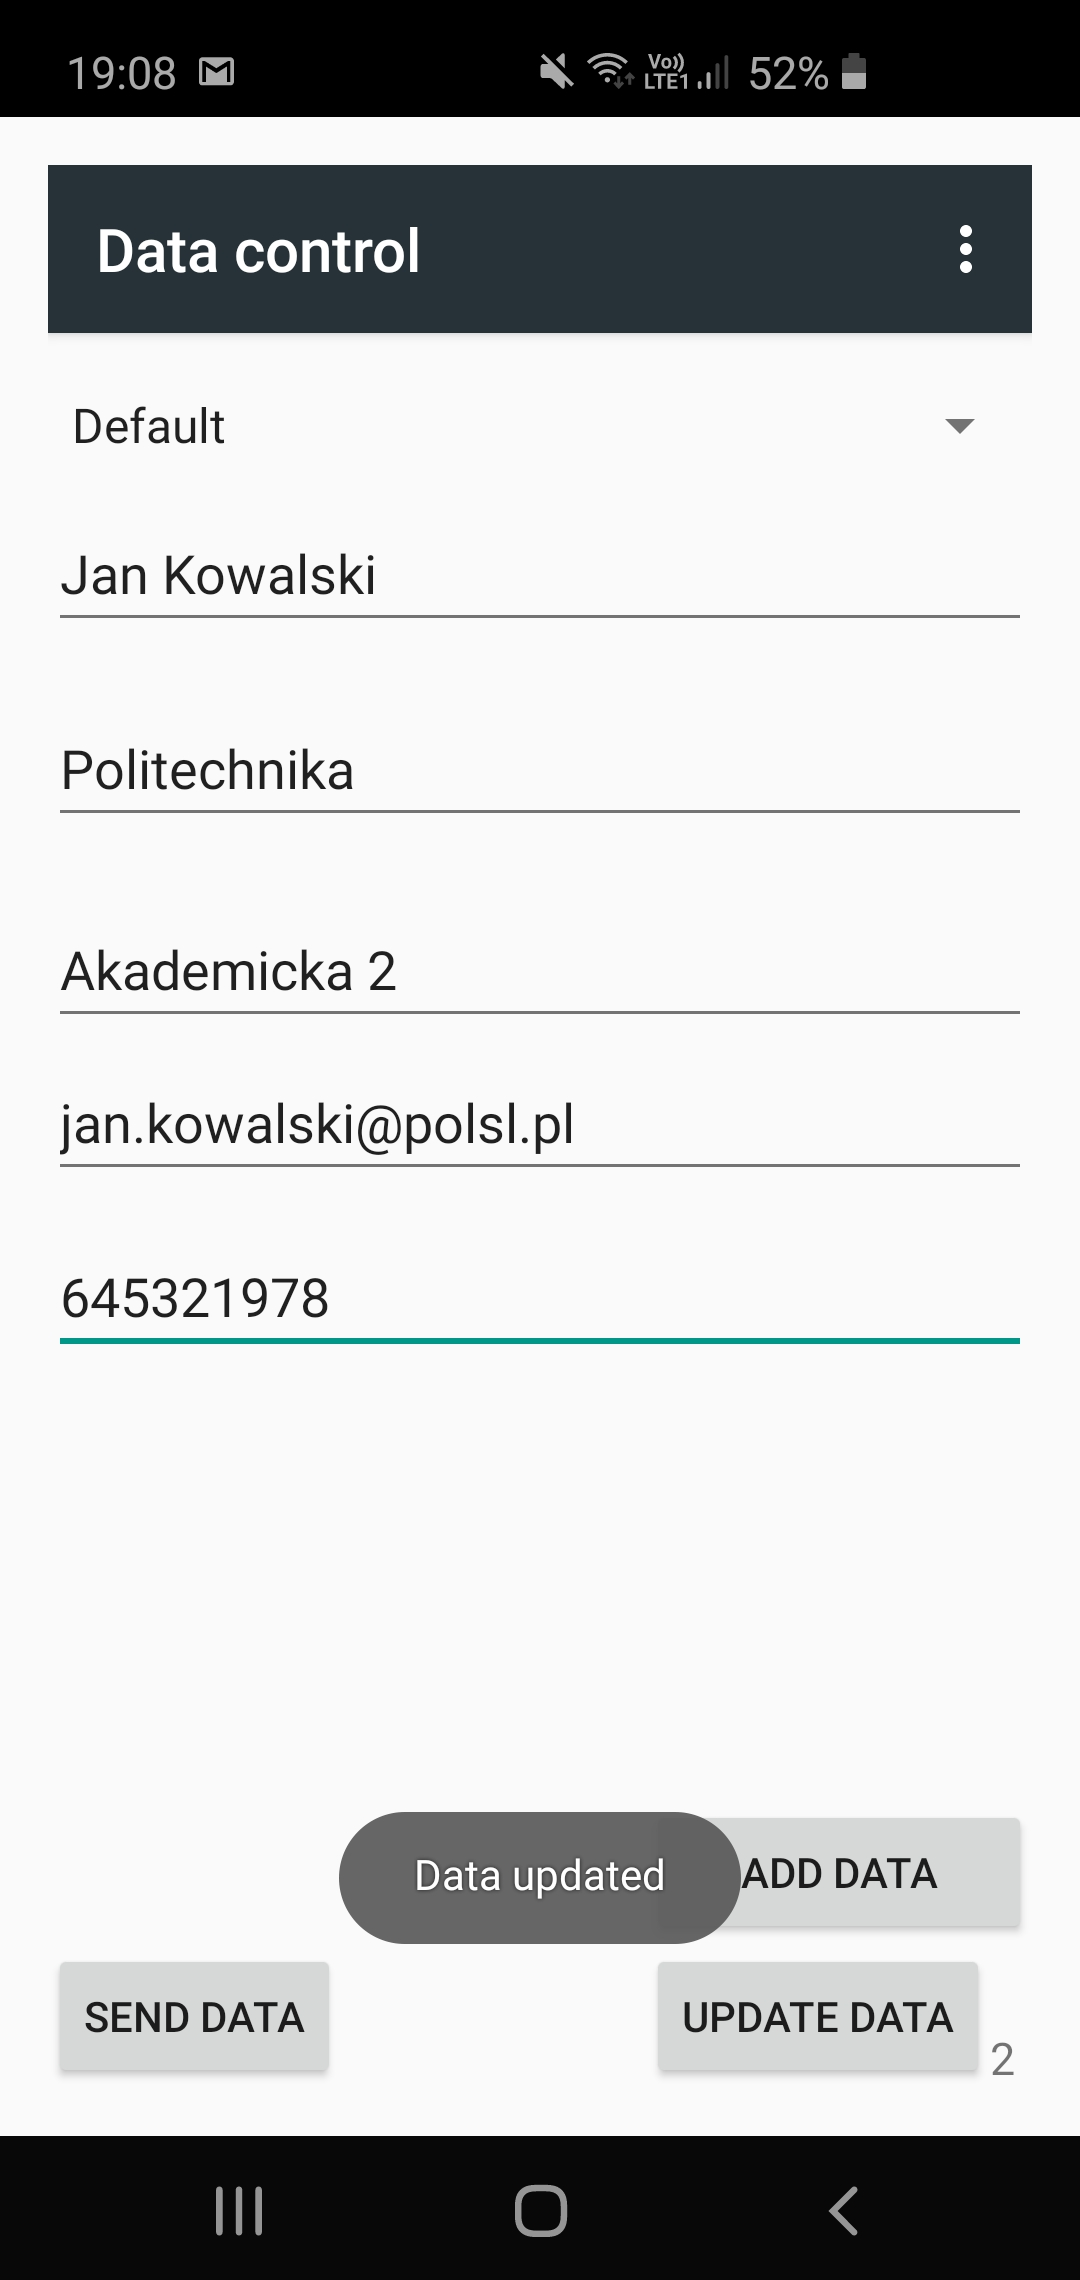
\includegraphics[width=5cm]{images/view_dataEdit.jpg}
    	            \captionof{figure}{Ekran po wczytaniu danych z~listy}
                    \label{fig:dataEdit}
                \end{minipage}
    	   \end{figure}
    	   Przycisk \textit{SEND DATA} odpowiada za przesyłanie umieszczonych w~polach edycyjnych danych na ekran plakietki. Po jego wciśnięciu pobierana jest zawartość pól edycyjnych i~identyfikator wybranego w~spinnerze layoutu, które przekazywane są do metody wysyłającej dane do plakietki. Layouty wyświetlane w~spinnerze pobierane są z~bazy danych. W~aktywności obsługi danych zostały również umieszczone przyciski do interakcji z~tabelą wpisów danych. Po wciśnięciu przycisku \textit{ADD DATA} do bazy danych zostaje dodany nowy rekord z~zawartością pól edycyjnych i~aktualnie wybranym layoutem. Edycja danych po wciśnięciu przycisku \textit{UPDATE DATA} dostępna jest dopiero po wcześniejszym wybraniu layoutu z~aktywności \textit{Data list} zawierającej element RecyclerView z~listą danych. Po powrocie do aktywności \textit{Data control}, w~prawym dolnym rogu uzupełniony zostanie element ID, dzięki czemu wiadomo, który element jest edytowany.
    	   \item \textbf{Data list} — jest to aktywność do prezentacji zapisanych w~urządzeniu wpisów danych osobowych. Głównym elementem jest RecycleView, na którym prezentowane jest imię i~nazwisko danej osoby oraz nazwa firmy. Dane pobierane są z~bazy danych.  
    	   \begin{figure}[H]
    	        \centering
    	        \begin{minipage}{.5\textwidth}
                    \centering
    	            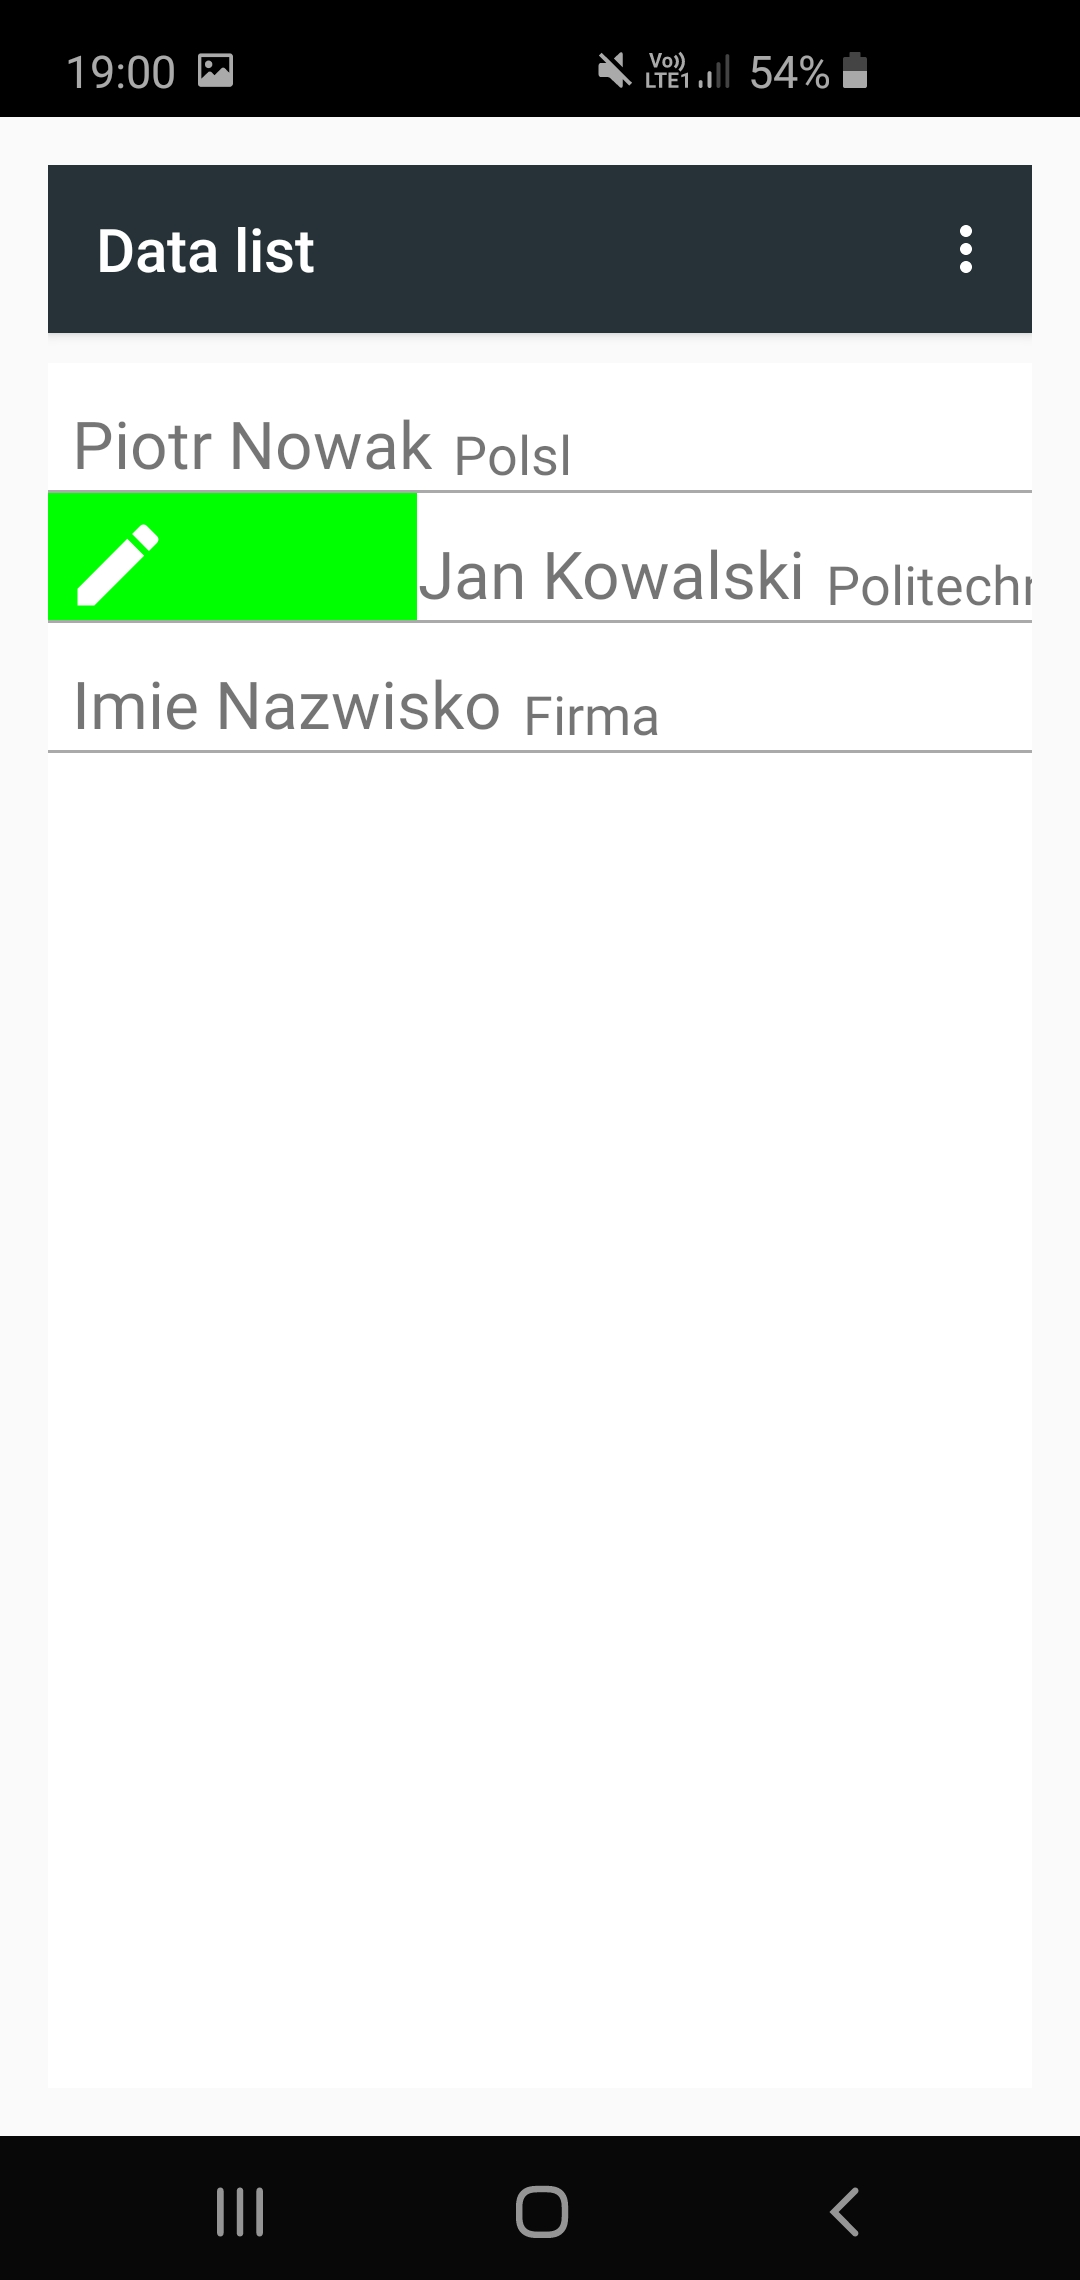
\includegraphics[width=5cm]{images/view_dataList.jpg}
    	            \captionof{figure}{Lista danych — edycja}
                    \label{fig:datalist}
                \end{minipage}%
    	        \begin{minipage}{.5\textwidth}
    	            \centering
    	            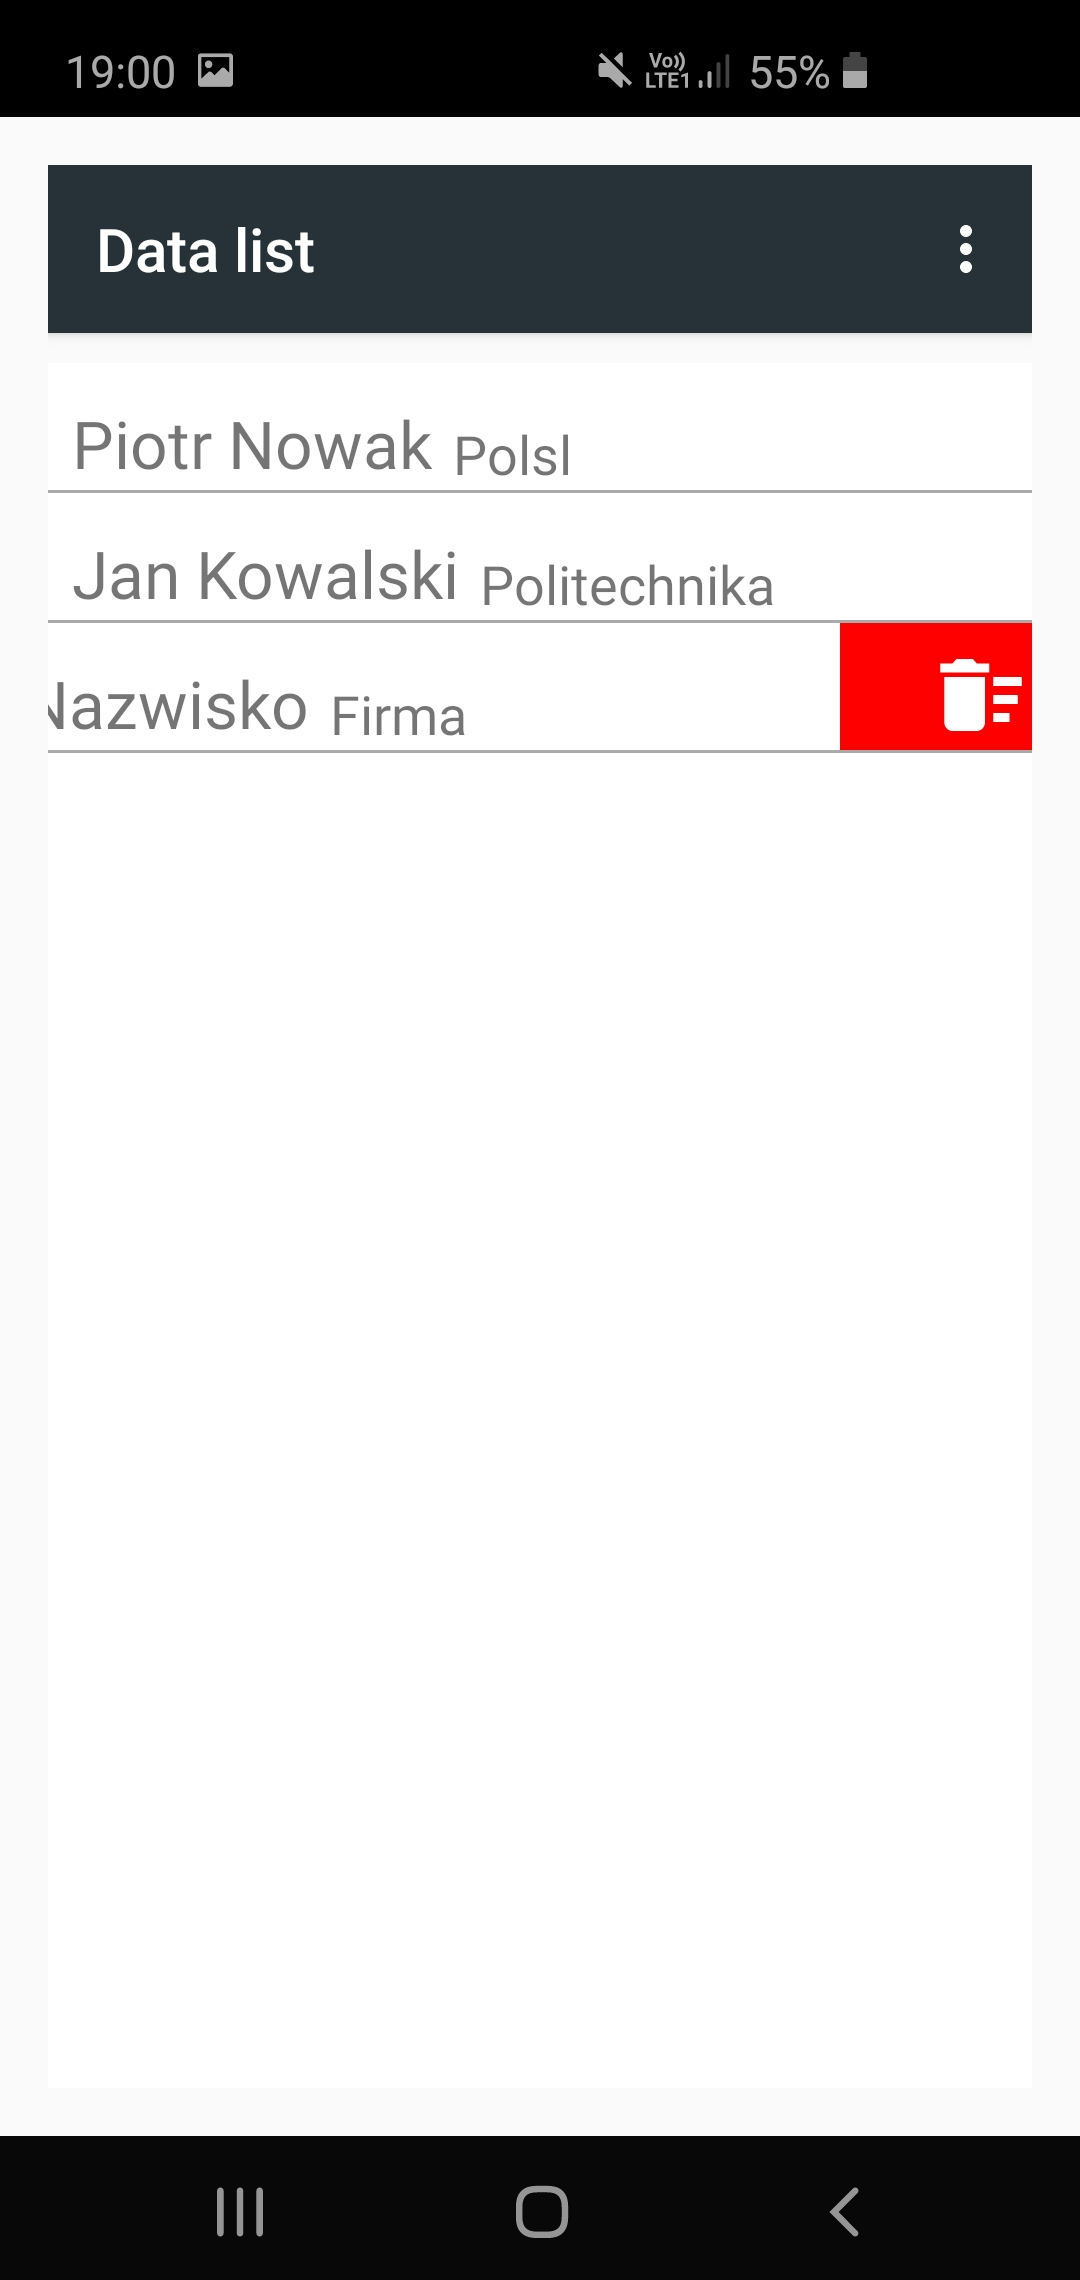
\includegraphics[width=5cm]{images/view_dataRemove.jpg}
    	            \captionof{figure}{Lista danych — usuwanie}
                    \label{fig:datadelete}
                \end{minipage}%
    	   \end{figure}
    	   Zaimplementowane metody usuwania rekordu i~edycji danych dostępne są po przesunięciu wpisu. W~trakcie przesuwania rekordu prezentowane jest graficzne przedstawienie akcji, która zostanie wykonana. Przesunięcie w~lewo skutkuje usunięciem wpisu z~bazy danych. Tło pod wierszem zmienia kolor na czerwony i~wyświetlana jest ikona kosza. 
    	   Po przesunięciu w~prawo ukaże się nam ikona edycji danych i~zielone tło. Po pełnym przesunięciu w~prawo przechodzimy do aktywności \textit{Data control}, gdzie pola edycyjne uzupełnione są danymi przesuniętego rekordu. Zgodnie z~danymi w~bazie danych dla konkretnego wpisu wybierany jest layout i~uzupełniane zostaje pole wyświetlające identyfikator rekordu. Odblokowana zostaje funkcjonalność edycji danych. Menu daje dostęp przełączenia się do widoku listy layoutów. 
    	   \item \textbf{Layout control} — aktywność ta wykorzystywana jest do tworzenia i~edycji wzorców układów wyświetlania danych. Umieszczone są tu przyciski opcji wyboru orientacji, jednocześnie może być aktywny tylko jeden z~nich. Przełączenie jednego do stanu aktywności, powoduje odznaczenie drugiego. Znajduje się tu również pole edycji nazwy layoutu oraz pola służące do wyboru współrzędnych miejsca, w~których mają zostać wyświetlone informacje. Każda z~możliwych do wyświetlenia danych (imię i~nazwisko, nazwa firmy, adres, email i~numer telefonu) posiada swoje pola edycji współrzędnych. Dla każdej informacji jest również dostępny przełącznik wyboru rozmiaru czcionki. Przełącznik nieaktywny oznacza wybór mniejszej, 9 punktowej, czcionki. Aktywny przełącznik oznacza większa czcionkę, 12 punktową. Z~dostępnego menu możliwe jest przejście do listy dostępnych layoutów. 
    	   \begin{figure}[H]
    	        \centering
    	        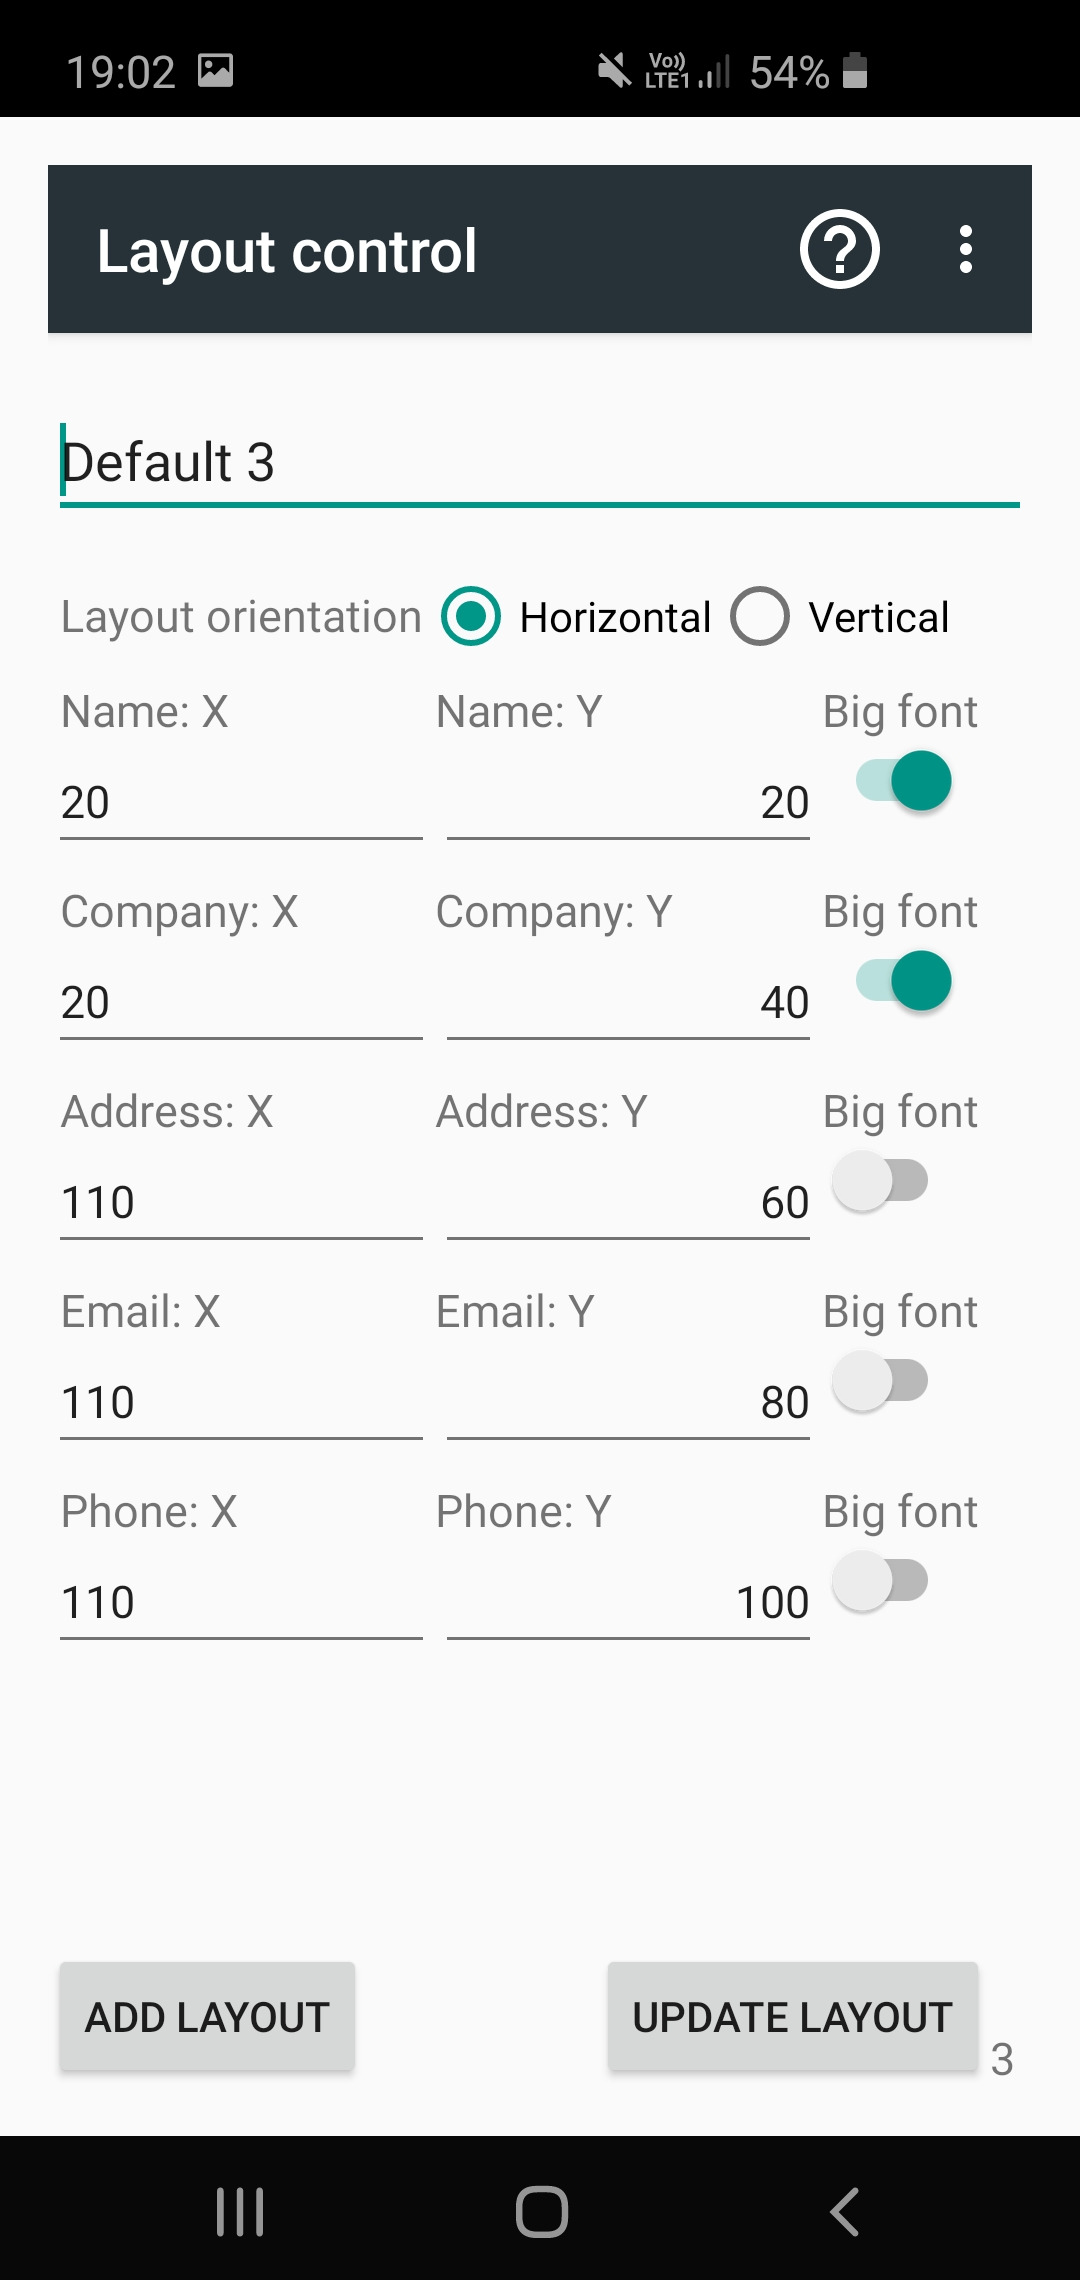
\includegraphics[width=5cm]{images/view_layoutEdit.jpg}
    			\caption{ Ekran dodawania i~edycji layoutów}
                \label{fig:layoutControl}
    	   \end{figure}
    	   Ikona pytajnika jest przyciskiem otwierającym dialog pomocy. Prezentowane w nim zasady i~wskazówki dotyczące dodawania nowych wzorców wyświetlania danych. Przedstawiony jest tam przykładowy ekran wyświetlacza, uzupełniony danymi i~wyświetlonymi wartościami użytego layoutu.
    	   Dostępne są tutaj również dwa przyciski działające analogicznie z~przyciskami znajdującymi się w~aktywności \textit{Data control}. Przycisk \textit{ADD LAYOUT} zapisuje do bazy nowy layout z~wartościami wprowadzonymi do elementów widocznych na ekranie. Przycisk \textit{UPDATE LAYOUT} staje się dostępny po wybraniu elementu z~listy layoutów i~używany jest do edycji wybranego layoutu.
    	   
           \item \textbf{Layout list} — aktywność ta służy do prezentacji zapisanych w~bazie danych wzorców układów prezentowanych danych. Elementem na którym prezentowane są dane jest RecycleView. Dla każdego wyświetlanego rekordu layoutu prezentowana jest nazwa układu i~jego identyfikator. Zaimplementowana jest metoda usuwania, dostępna po przesunięciu rekordu w~lewo. Dostępna jest również funkcjonalność edycji layoutu, która aktywuje się po przesunięciu wiersza w prawo. Po wykonaniu akcji edycji aplikacja przenosi użytkownika do aktywności \textit{Layout control}, gdzie w~pola edycyjne zostają wprowadzone dane wybranego układu. Uzupełnione zostaje pole ID i~odblokowane jest edytowanie układu. 
           \begin{figure}[H]
    	        \centering
    	        \begin{minipage}{.5\textwidth}
                    \centering
    	            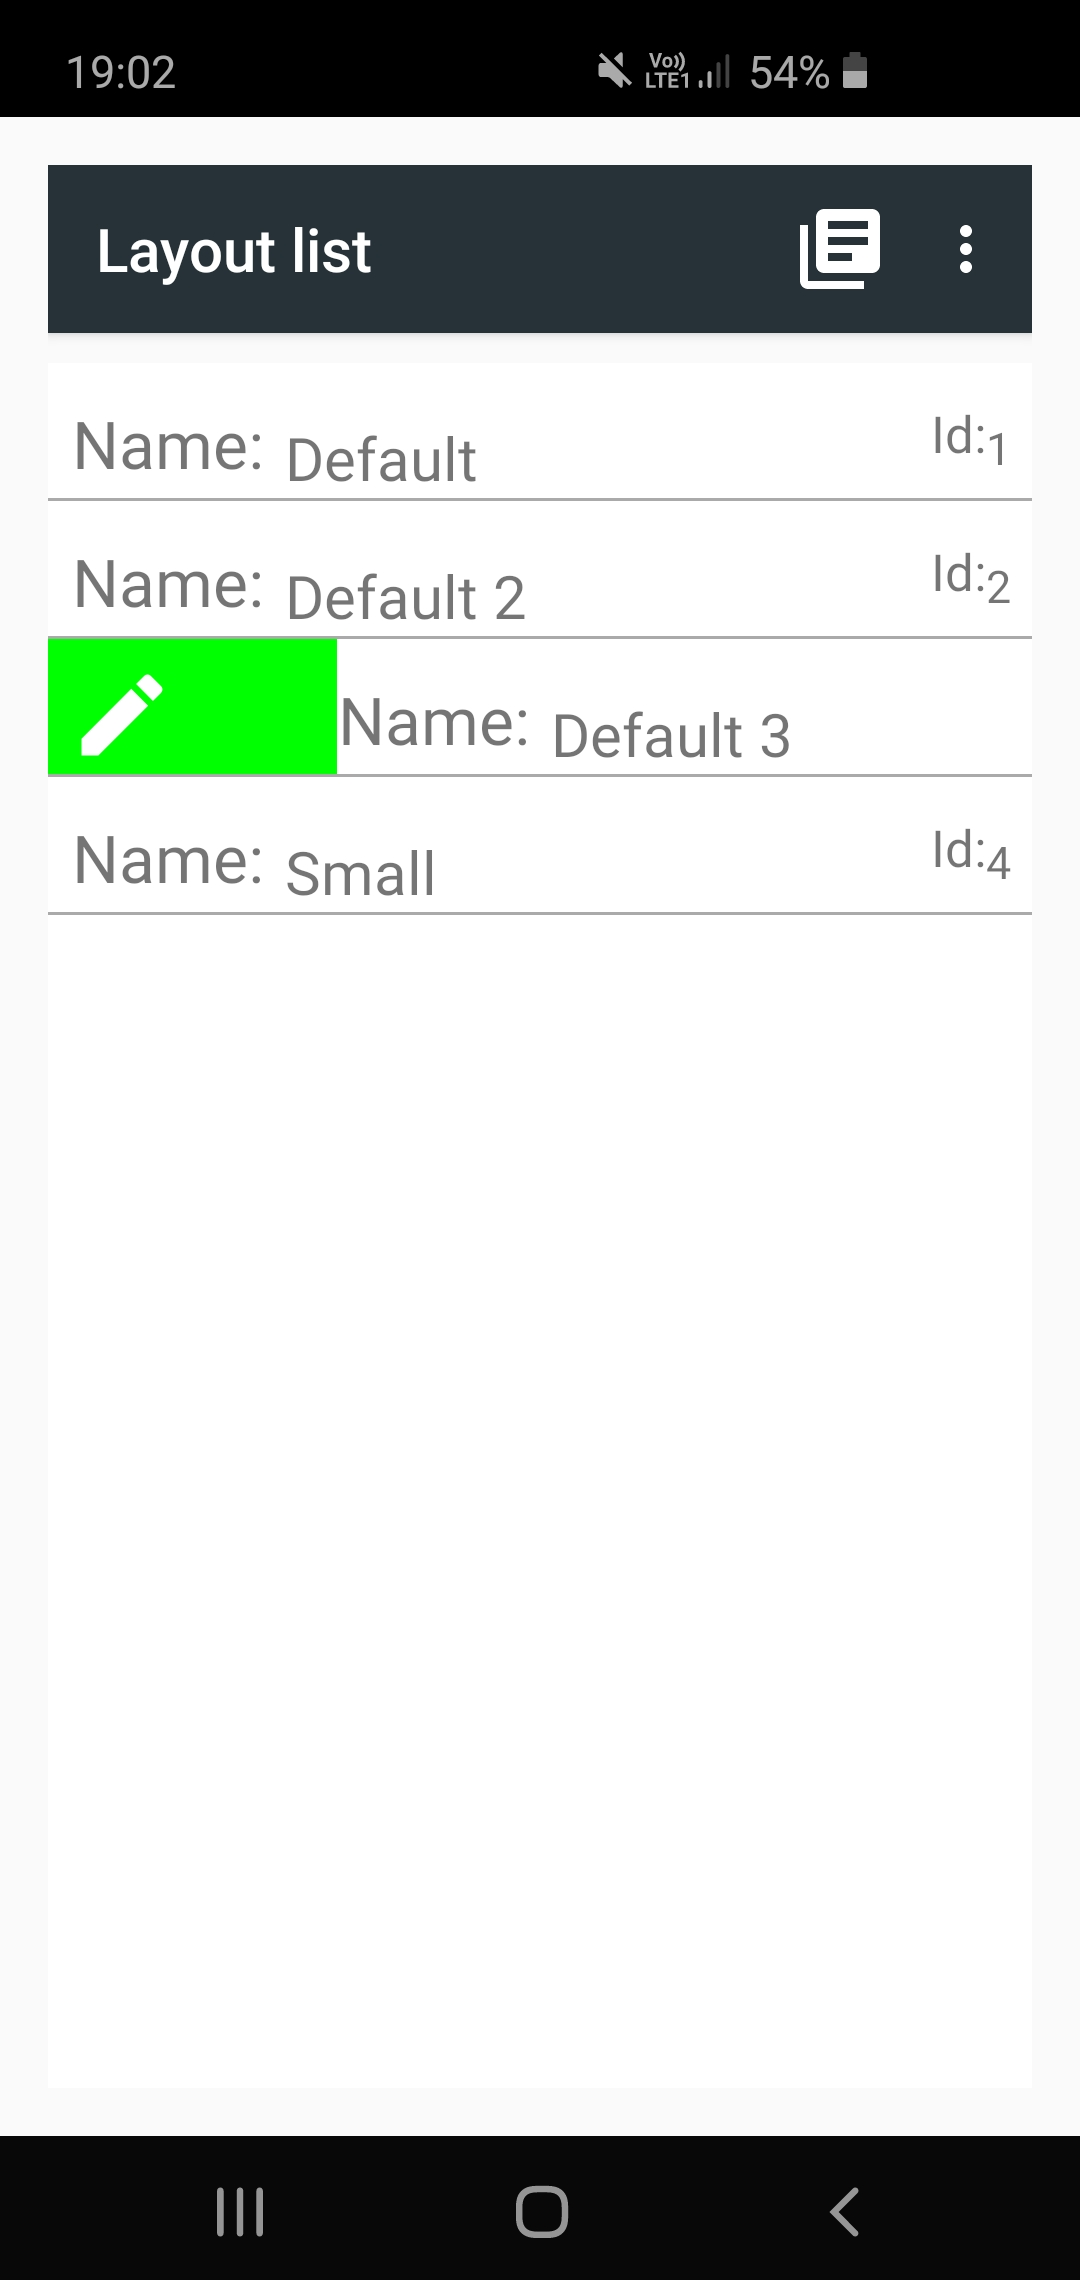
\includegraphics[width=5cm]{images/view_layoutList.jpg}
    	            \captionof{figure}{Lista układów — edycja}
                    \label{fig:layoutlist}
                \end{minipage}%
    	        \begin{minipage}{.5\textwidth}
    	            \centering
    	            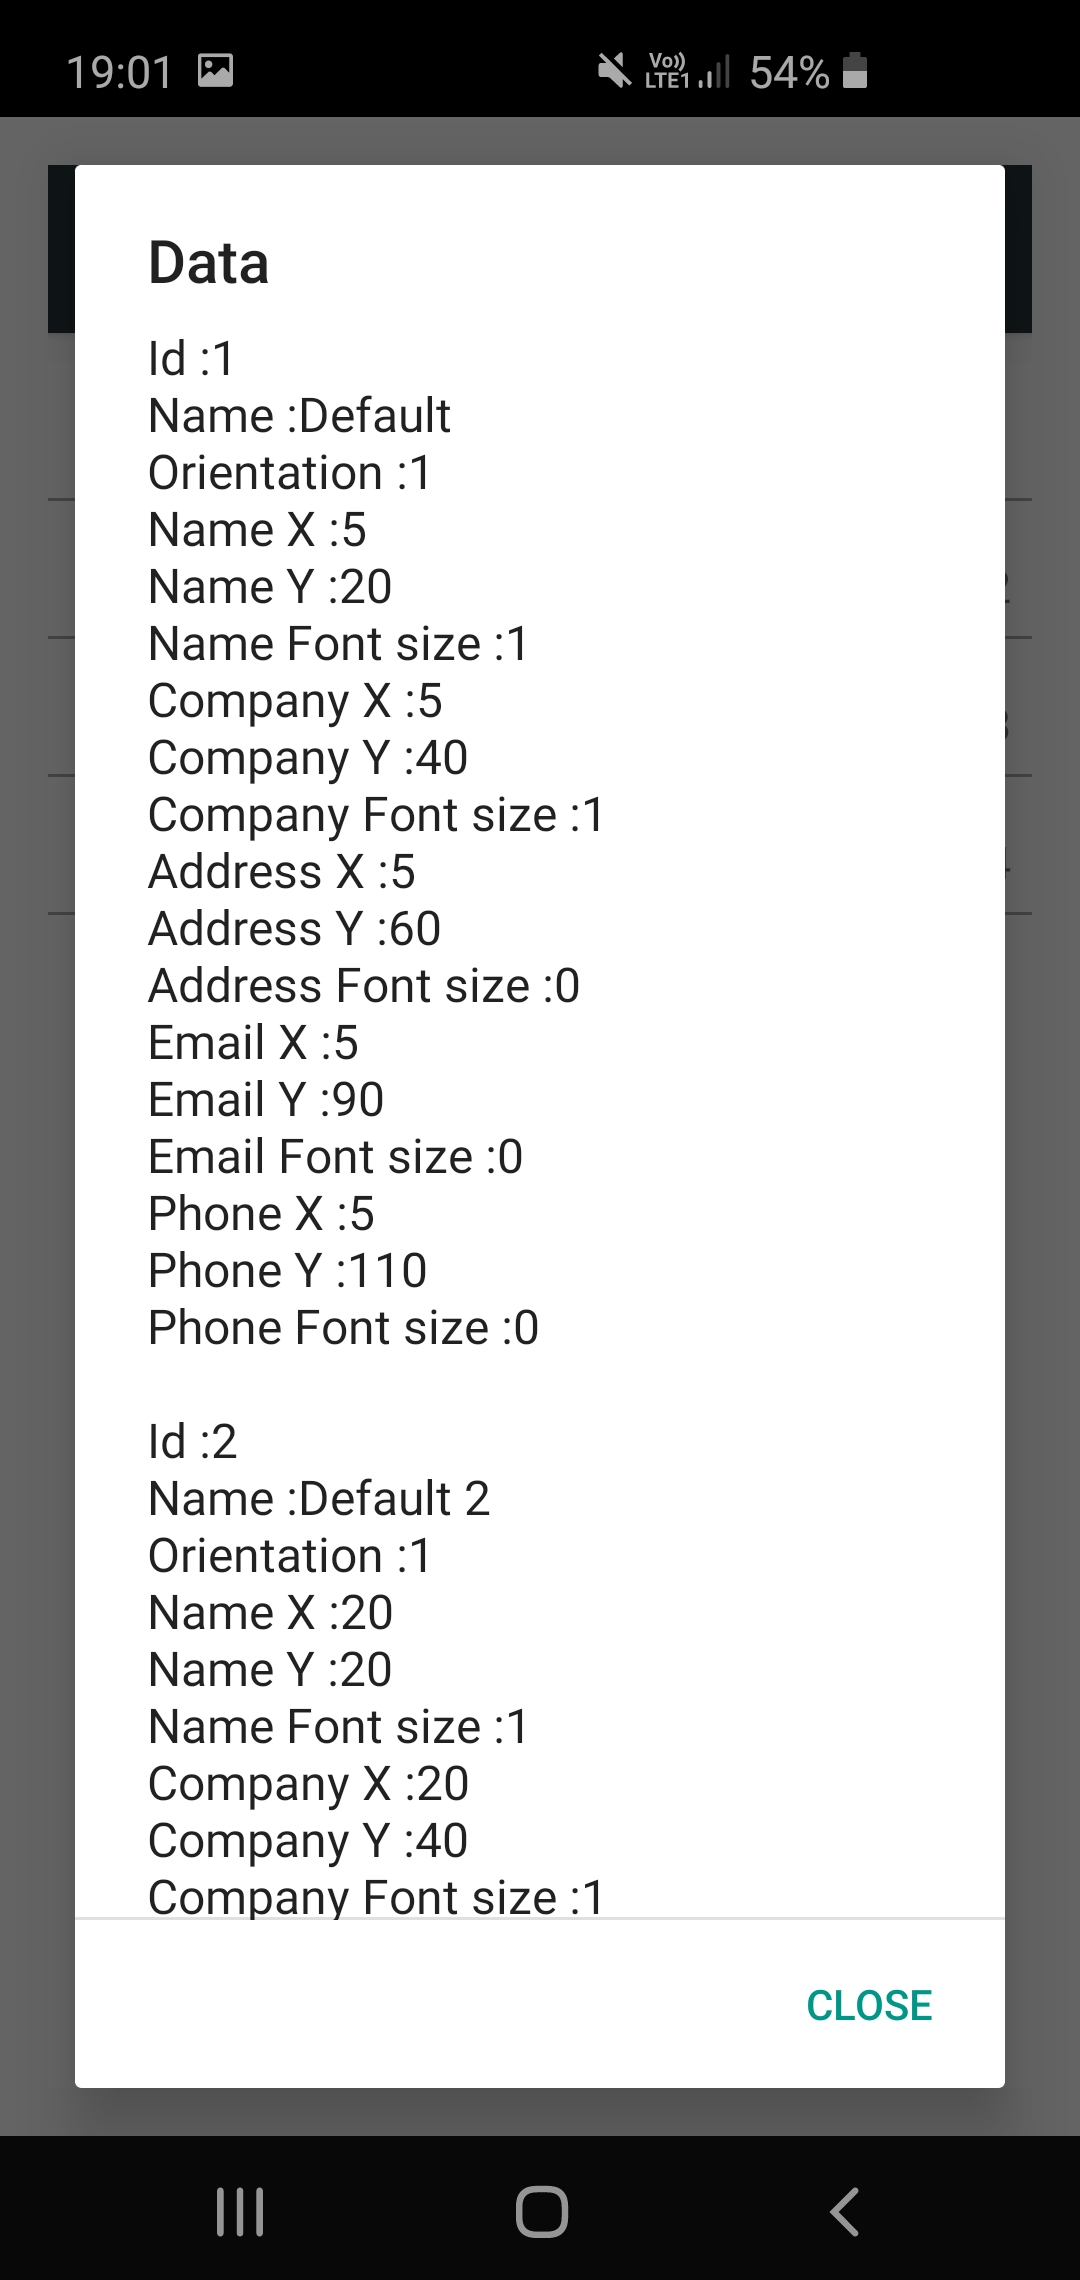
\includegraphics[width=5cm]{images/view_layoutDetails.jpg}
    	            \captionof{figure}{Lista układów — szczegóły}
                    \label{fig:layoutlistDialog}
                \end{minipage}%
    	   \end{figure}
           Do prezentacji szczegółów wzorcu układu służy przycisk mieszczący się w~menu aktywności. Po jego wciśnięciu wyświetlony zostaje dialog pokazany na rysunku \ref{fig:layoutlistDialog}, na którym wyświetlane są wszystkie wartości elementów znajdujących się w~bazie danych. Z~rozwijanego menu istnieje także możliwość przejścia do aktywności dodawania layoutów.
           
    	\end{enumerate}
    	
    	Każda aktywność posiada również w~swoim rozwijanym menu możliwość wyświetlenia informacji o~aplikacji i~autorze.
 
        \subsection{Baza danych}
        W~aplikacji istnieje możliwość przechowywania rekordów zapisanych wpisów z~danymi personalnymi oraz układów danych. Obsługa zapisanych danych wykonywana jest w~relacyjnej bazie danych SQLite. Baza posiada dwie tabele połączone ze sobą kluczem obcym. Na rysunku numer \ref{fig:database}. można zobaczyć diagram związków encji bazy danych. 
        
        Kolumna id występująca w~tabeli \textit{layouts} jest kluczem głównym tej tabeli. Wykorzystywana jest również jako klucz obcy tabeli \textit{data}. 
        
        \begin{figure}[H]
    	        \centering
    			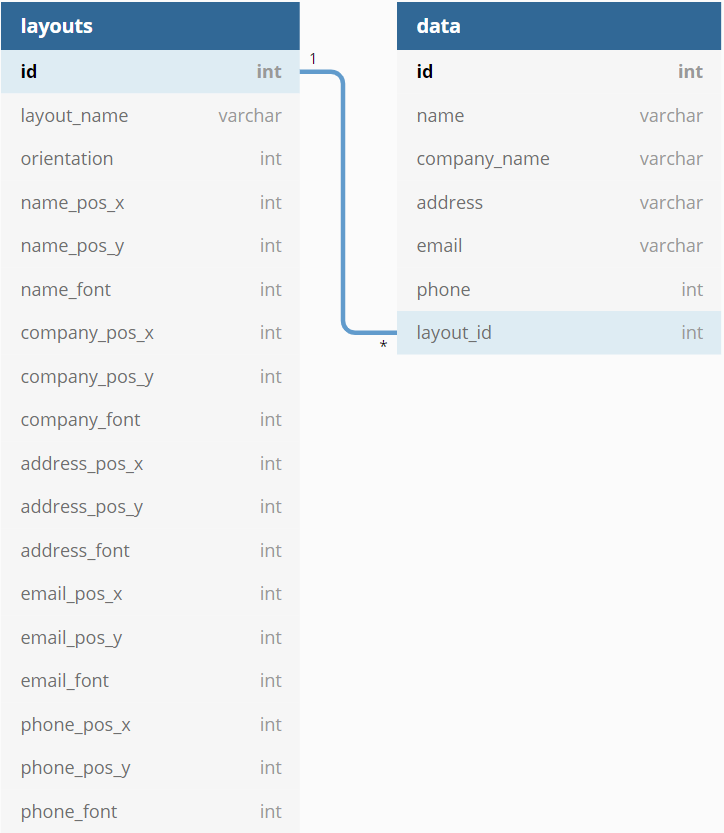
\includegraphics[width=9cm]{images/rys_11baza.png}
    			\caption{Diagram związków encji bazy danych}
                \label{fig:database}
    	\end{figure}
    	
        Relacja występująca pomiędzy tabelami to relacja jeden do wielu (1: N). Oznacza to, że jeden rekord tabeli \textit{layouts} może być wykorzystany przez wiele rekordów w~tabeli \textit{data}. Z~drugiej strony, pojedynczy wpis w~tabeli \textit{data} może posiadać tylko jeden layout. Dzięki takiemu połączeniu SQLite zapewnia poprawność działania bazy danych, uniemożliwiając usunięcie wpisów wykorzystywanych przez inne tabele. 
        
        W~zaprojektowanej dla projektu bazie danych niemożliwe będzie usunięcie rekordu tabeli \textit{layouts}, gdy jego klucz główny \textit{id} jest obecny w~kolumnie \textit{layout\_id} tabeli \textit{data}, który jest kluczem obcym tej tabeli. Po wykryciu przez bazę danych takiego zachowania zwracany jest błąd, który następnie zostaje obsłużony przez aplikację w~celu przekazania użytkownikowi informacji o~niepożądanej akcji.
        
        \subsection{Opis funkcjonalności}
    	
    	\subsubsection{Algorytm wysyłania danych}
    	Wysyłanie danych do mikrokontrolera możliwe jest tylko w~aktywności \textit{Data control}. Występuje w~niej przycisk, po wciśnięciu którego wykonywana jest procedura przesłania danych do mikrokontrolera. Pierwszym krokiem jest pobranie zawartości pól edycyjnych, w~których umieszczone są informacje do wyświetlenia i~zapisywanie ich do zmiennych. Zmienne te razem z~identyfikatorem wybranego layoutu, dalej layoutId, przesyłane są jako argumenty do funkcji, która pobiera z~tabeli \textit{layouts} wartości rekordu o~przesłanym identyfikatorze.
    	
    	Posiadając wszystkie informacje niezbędne do przesłania, zostaje rozpoczęta procedura dodawania wszystkich zmiennych w~jeden ciąg znaków. Jako pierwsza znajduje się wartość oznaczająca orientację wyświetlacza. Następnie przesyłane są współrzędna X, współrzędna Y, wartość do wyświetlenia, te 4 wartości powtarzane są dla każdego elementu, który może być wyświetlony. Pomiędzy każdą zmienną wstawiany jest średnik, który w~mikrokontrolerze wykorzystany jest do zdekodowania ciągu znaków. Poniżej przedstawiono przykładowy ciąg znaków po zakodowaniu.
    	\begin{lstlisting}[language=C++, label={lst:przykladowePrzesylaneDane}, caption=Przykładowy ciąg przesyłanych danych]
O X  Y F DATA X  Y F DATA  X Y  F DATA  X Y  F DATA  X Y   F DATA	
1;5;20;1;Imie;5;40;1;Firma;5;60;0;Adres;5;90;0;Email;5;110;0;65467819;
gdzie:  O~- orientacja
        X - wartosc wspolrzednej X
        Y - wartosc wspolrzednej Y
        F - okresla rozmiar czcionki
        DATA - przesylane dane\end{lstlisting}
    
    	Po przygotowaniu danych w~taki sposób zostają one przesłane przez nawiązane z~mikrokontrolerem połączenie Bluetooth.

    	Obsługa przesyłania danych realizowana jest poprzez klasę \textit{BluetoothSocket}. Używając metody \textit{getOutputStream}\cite{outputstream}, otwarty zostaje strumień wyjścia, za pomocą którego przesyłane są dane. Algorytm służący do dekodowania odebranych przez urządzenie mobilne danych, obecny jest w~mikrokontrolerze i~został opisany w~części \ref{petladekod} \textit{Opis części programowej mikrokontrolera}.
    	
    	Transmisja danych możliwa jest tylko w~wypadku, gdy gniazdo Bluetooth jest połączone z~urządzeniem docelowym.
	
    	\subsubsection{Konstruowanie layoutu}
    	Przed rozpoczęciem konstrukcji layoutu należy posiadać wiedzę na temat wykorzystanej w~projekcie czcionki i~rozmiarów pojedynczego znaku, aby uniknąć tworzenia układów, w~których dane na siebie nachodzą. W~projekcie wykorzystane są dwie czcionki FreeMono9pt7b i~FreeMono12pt7b. W~przypadku mniejszej czcionki przestrzeń potrzebna do wyświetlenia znaku wynosi 11x18 pikseli. Większa z~nich ma wymiary 14x24 pikseli dla pojedynczego znaku.
    	\begin{figure}[H]
    	        \centering
    			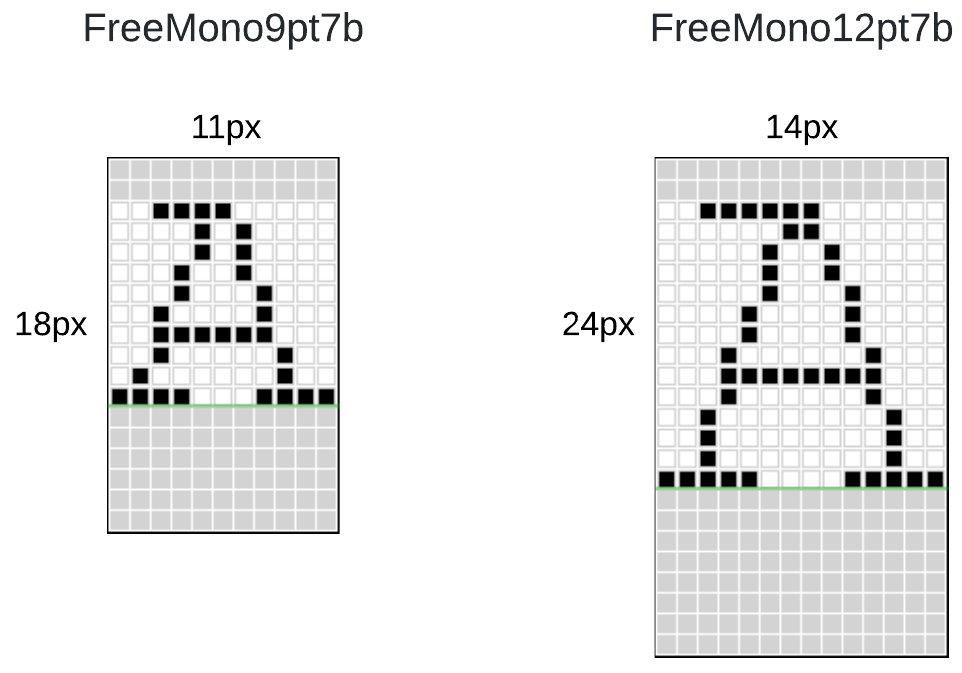
\includegraphics[width=8cm]{images/rozmiarczcionek.png}
    			\caption{Rozmiary pojedynczego znaku czcionki}
                \label{fig:font}
    	\end{figure}
    	
    	Znając wymiary pojedynczego znaku można określić maksymalną ilość znaków, które zmieszczą się w~jednej linii. Wykorzystany w~projekcie wyświetlacz posiada 296 pikseli. Co dla czcionki 9 punktowej oznacza ilość pojedynczych znaków równą 26. W~przypadku większej czcionki ograniczenie wynosi 21 znaków.
    	
    	W płaszczyźnie Y chcąc wyświetlać różne dane linijka pod linijką powinno zostawić się co najmniej 18, 24 pikseli wolnego miejsca w~zależności od wybranej czcionki.
    	
    	W płaszczyźnie X trzeba również zwrócić uwagę na ilość znaków, które chcemy wyświetlić dla danej informacji. Przy zamierzeniu wyświetlania 10 znaków informacji, kolejna informacja powinna być oddalona o~co najmniej \([(ilosc + 1)*szerokosc]\) pikseli. Wartość, którą mnożymy przez szerokość znaku jest liczba znaków powiększona o~jeden dla zachowania przerwy pomiędzy wyświetlanymi informacjami.\newline
    	
    	Na rysunku \ref{fig:sampleLayout} przedstawiony został ekran wyświetlacza z~wyświetlonymi przykładowymi danymi. Naniesione na niego zostały wartości dla wybranego layoutu. 'Imię Nazwisko' oraz  'Firmy' wyświetlane są z~użyciem 12 punktowej czcionki. Zostały oddalone od siebie o~24 punkty w~celu zachowania przejrzystości tekstu. 'Adres', 'Email' i~'numer telefonu' wyświetlane są 9 punktową czcionką. Odległość pomiędzy nimi wynosi 18 punktów. 
    	\begin{figure}[H]
    	        \centering
    			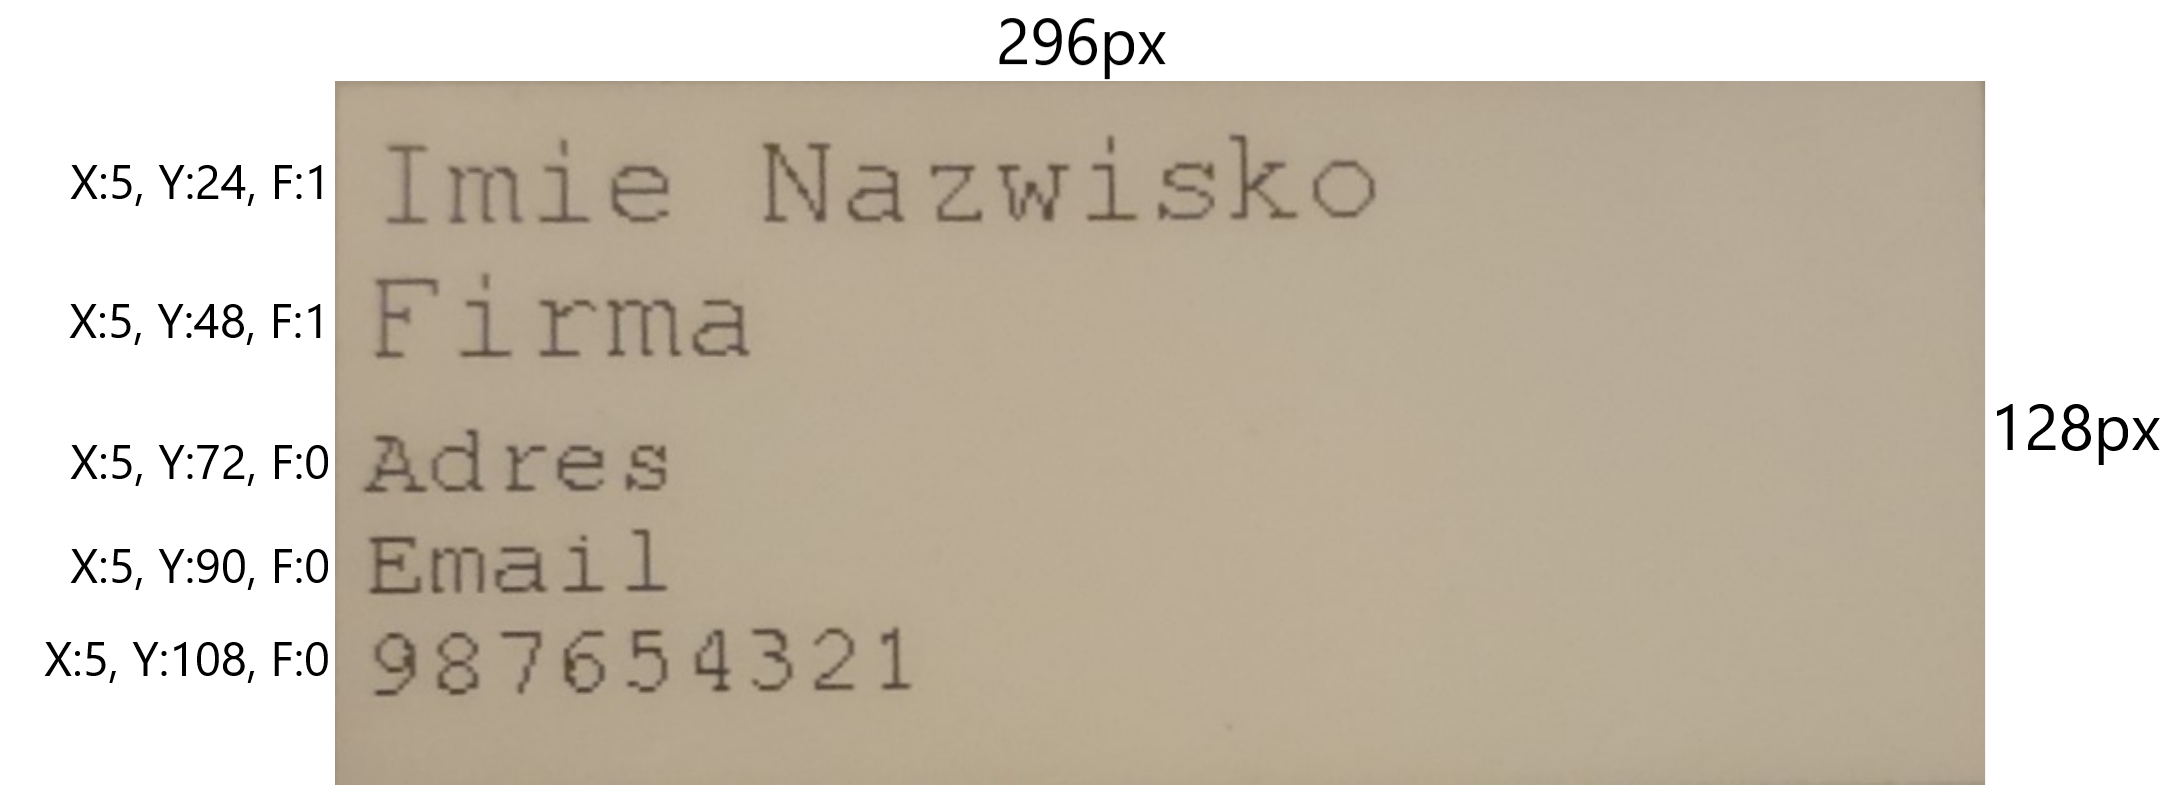
\includegraphics[width=13cm]{images/wygladlayout.png}
    			\caption{Przykładowe dane na wyświetlaczu z~pokazanymi wartościami użytego layoutu.}
                \label{fig:sampleLayout}
    	\end{figure}
    	
    	\subsection{Połączenie Bluetooth}
    	Połączenie, obsługa i~komunikacja Bluetooth są zarządzane poprzez pakiet dostępny dla systemu Android jakim jest \textit{android.bluetooth}\cite{android.bluetooth}. W~projekcie wykorzystywana jest funkcjonalność wyszukiwania dostępnych urządzeń, nawiązywania połączenia oraz przesyłania danych. Schemat blokowy przedstawiający nawiązywanie połączenia pomiędzy urządzeniem mobilnym a urządzeniem wyświetlającym, został ukazany na rysunku numer \ref{fig:btconnect}. 
    	\begin{figure}[H]
    	        \centering
    			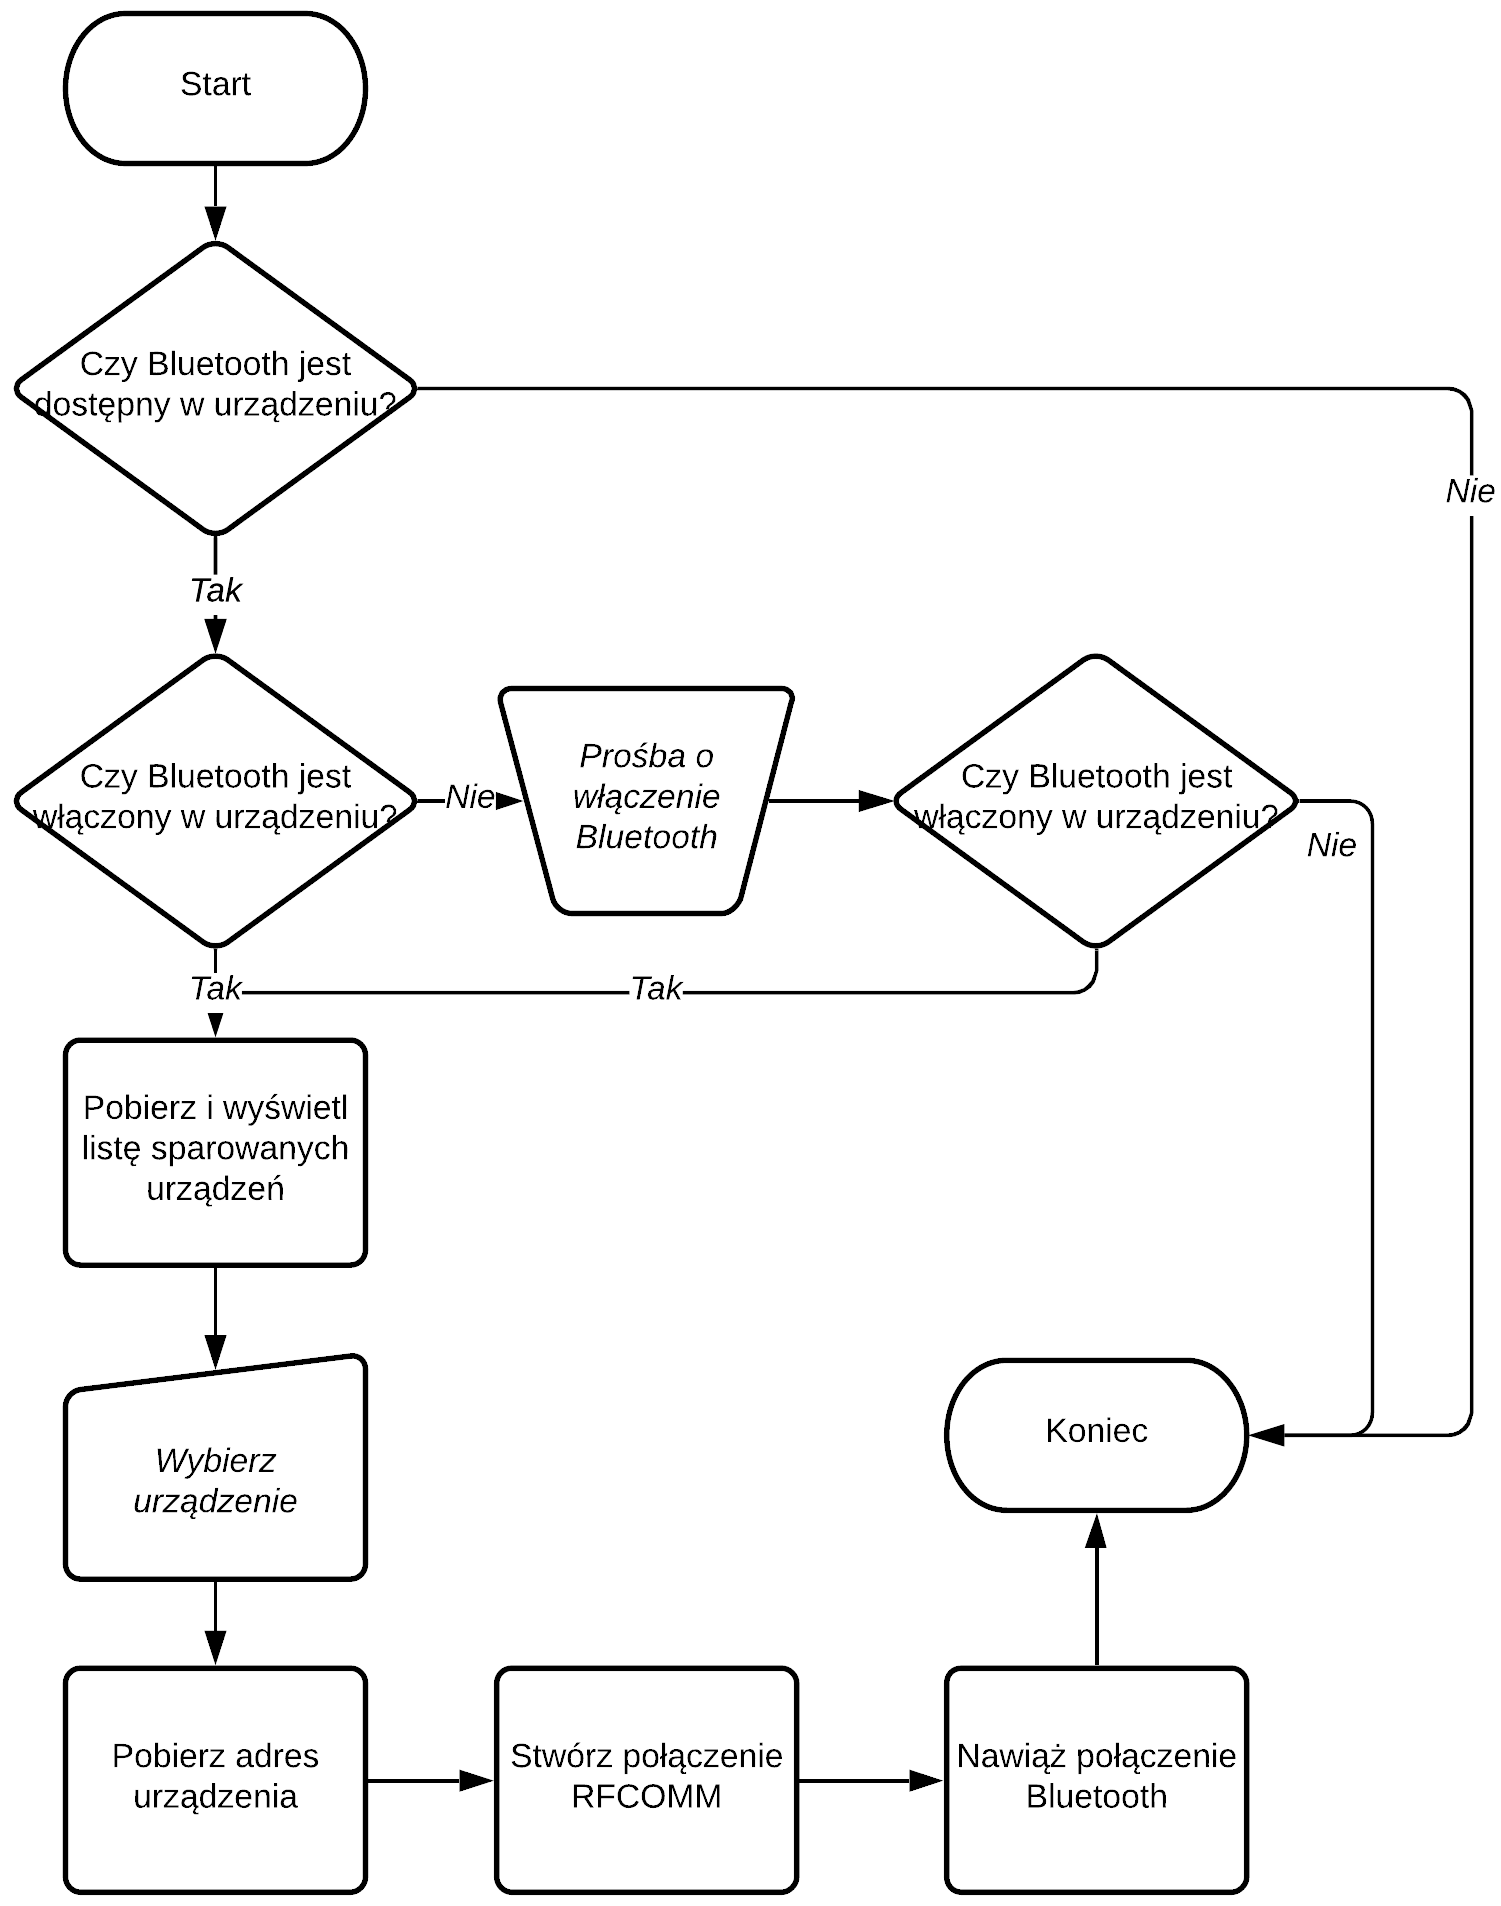
\includegraphics[width=12cm]{images/rys_12bluetoothconnection.png}
    			\caption{Schemat blokowy nawiązywania połączenia Bluetooth}
                \label{fig:btconnect}
    	\end{figure}
    	Pierwszym krokiem nawiązania komunikacji poprzez adapter Bluetooth jest sprawdzenie, czy moduł ten, jest obecny w~urządzeniu mobilnym. W~przypadku gdy urządzenie mobilne nie posiada adaptera Bluetooth, aplikacja blokuje większość funkcji, pozostawiając jedynie możliwość przeglądania i~dodawania nowych układów danych. 
    	
    	Przy pozytywnym stwierdzeniu obecności modułu, można przejść do dalszych kroków. Następnym etapem jest sprawdzenie czy moduł Bluetooth jest włączony. W~przypadku gdy Bluetooth jest wyłączony, następuje wyświetlenie prośby o~jego włączenie. Później pobierana jest lista sparowanych z~urządzeniem mobilnym urządzeń Bluetooth. Wykorzystano do tego metodę \textit{getBondedDevices}\cite{bonded} dostępną w~klasie \textit{BluetoothAdapter}. Metoda ta zwraca zbiór obiektów sparowanych z~lokalnym dla aplikacji adapterem Bluetooth. Po wybraniu urządzenia pobierany jest jego adres BD\_ADDR i~nawiązywana jest próba połączenia. Sprawdzana jest dostępność urządzenia, następnie utworzone zostaje połączenie \textit{RFCOMM} \cite{rfcomm}. Po wykonaniu poprzedzających czynności możliwe jest nawiązanie połączenia pomiędzy urządzeniami. Połączone urządzenia dysponują szeregowym połączeniem, po którym można przesyłać dane.
    	
    	
    	
    	\subsection{Konfiguracja aplikacji}
    	Przed pierwszym uruchomieniem aplikacji należy sparować urządzenie mobilne i~elektroniczną plakietkę ze sobą za pomocą łączności Bluetooth. Po upewnieniu się, że łączność Bluetooth w~naszym urządzeniu mobilnym jest włączona, można przejść do ustawień, gdzie należy znaleźć stronę z~ustawieniami połączeń Bluetooth. Po kliknięciu przycisku wyszukiwania urządzeń, wyświetlone zostaną dostępne do połączenia urządzenia. Należy znaleźć urządzenie o~nazwie \textit{ESP32test} i~połączyć się z~nim. Połączenie nie wymaga podania hasła lub pinu. Po sparowaniu urządzeń można przejść do uruchomienia aplikacji. 
    	
    	Po instalacji i~pierwszym uruchomieniu aplikacja tworzy bazę danych, która uzupełniana jest domyślnymi layoutami umożliwiającymi przesyłanie danych od razu po uruchomieniu i~konfiguracji urządzenia. Przy każdym włączeniu, sprawdzana jest obecność modułu Bluetooth. W~przypadku braku modułu, funkcjonalności aplikacji zostają ograniczone. Następnie sprawdzane jest czy moduł Bluetooth jest uruchomiony. Przy wyłączonym module aplikacja wyświetli dialog proszący o~włączenie modułu Bluetooth.
    	
    	\begin{figure}[H]
    	        \centering
    			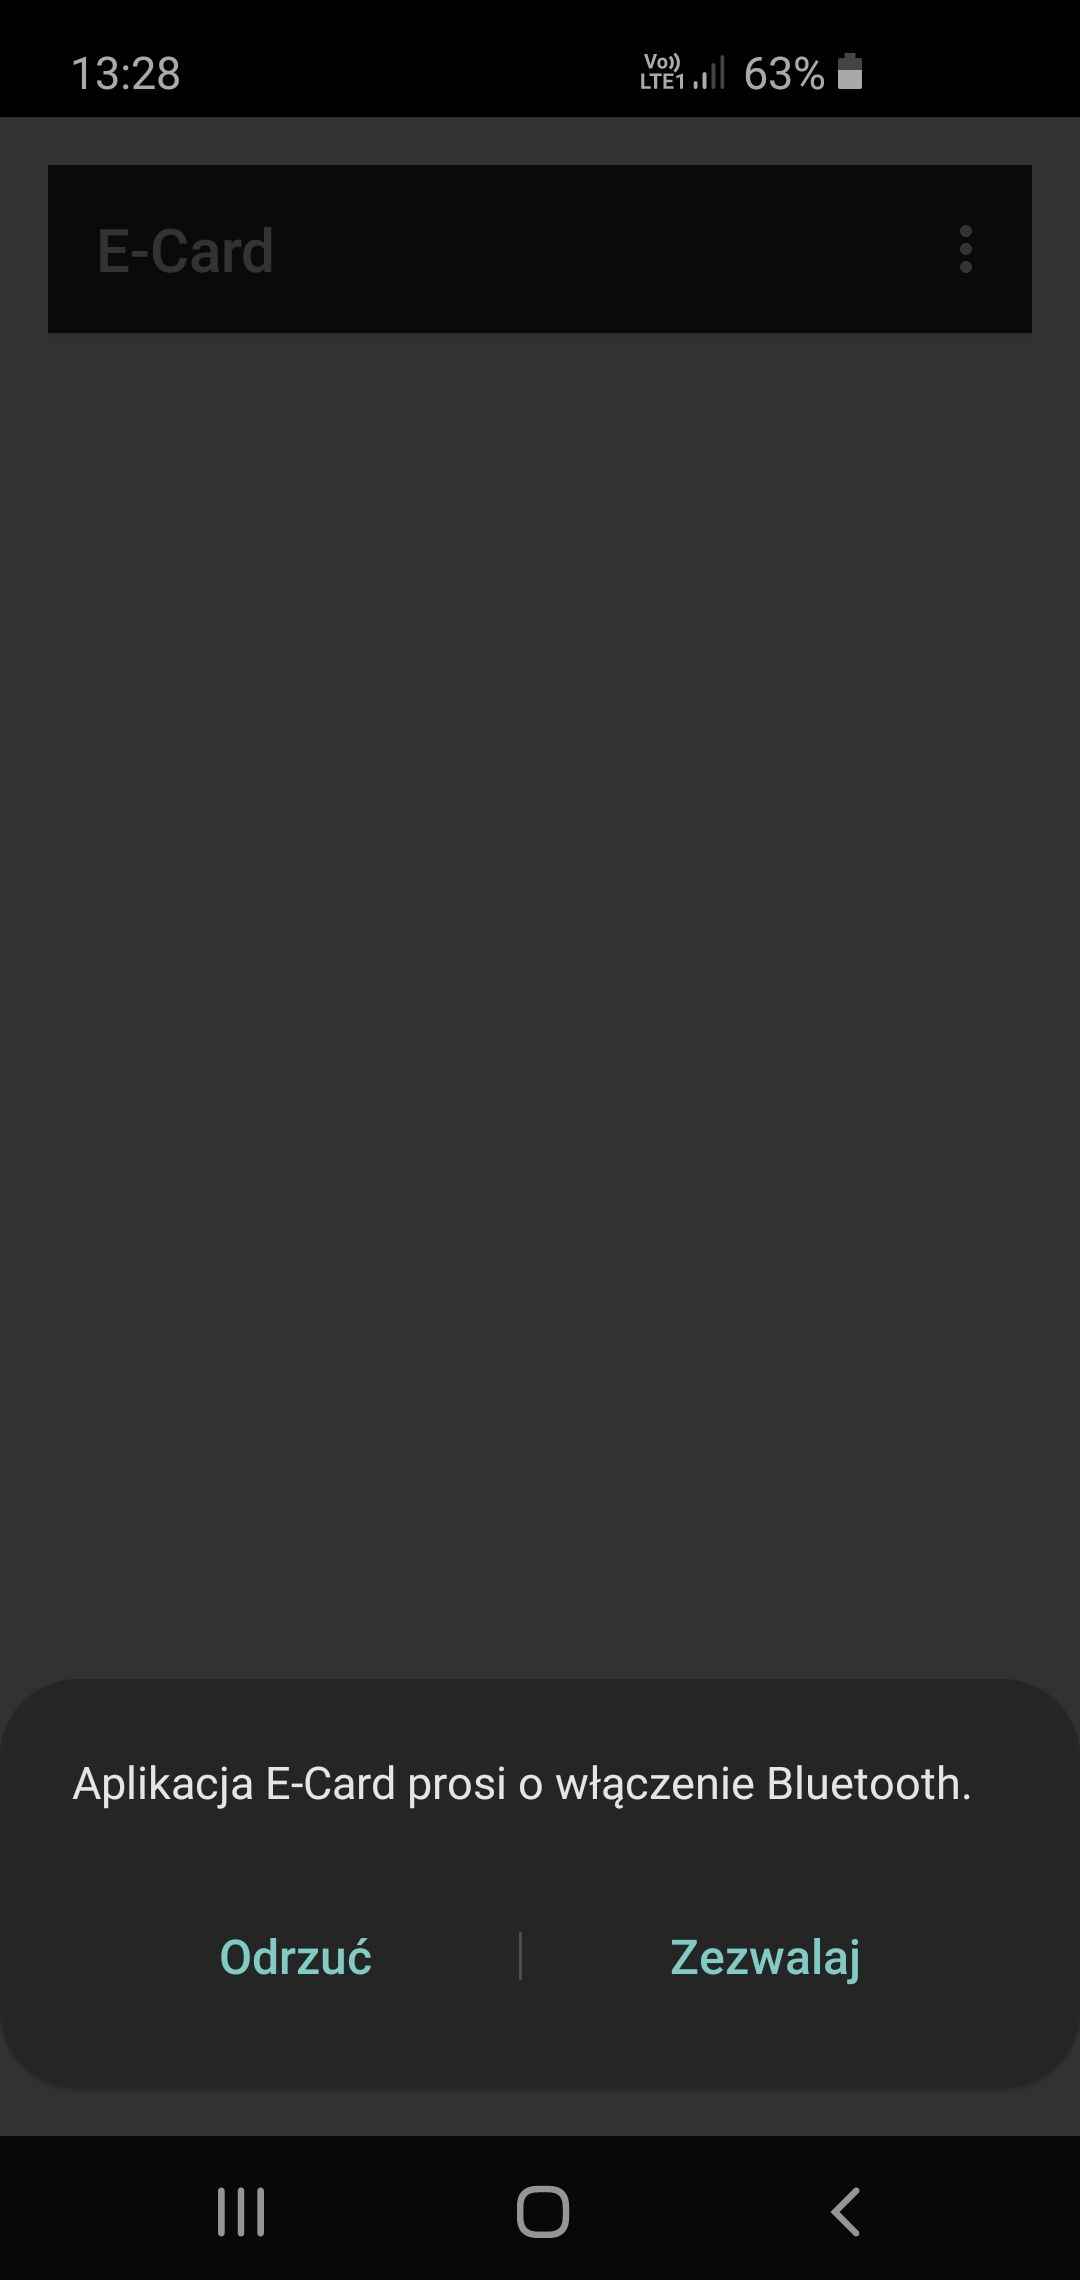
\includegraphics[width=5cm]{images/rys_13bluetoothdialog.jpg}
    			\caption{Dialog proszący o~włączenie Bluetooth}
                \label{fig:bton}
    	\end{figure}
    	
    	Po włączeniu adaptera Bluetooth wyświetlona zostaje lista urządzeń, z~którymi można się połączyć. Widok ten przedstawiono na rysunku numer \ref{fig:btdevices}. Po wybraniu nazwy prototypu, którą jest \textit{ESP32test}, aplikacja przechodzi do widoku sterowania danymi.
    	
    	Możliwości oferowane przez aplikację zostały opisane w~rozdziale \ref{podzialnaaktywnosci} \nameref{podzialnaaktywnosci}.
    	
    	\newpage
    	\section{Rozwój projektu}
    	Zbudowany prototyp poddany został praktycznym testom wszystkich funkcjonalności. W~trakcie testów badano sposób zachowania się aplikacji w~różnych wariantach działania i~na kilku różnych urządzeniach. Sprawdzono również poprawność pracy mikrokontrolera i~poprawność wyświetlania danych na ekranie.
    	
    	W trakcie testowania programu w~emulatorze, dostępnym w~środowisku Android Studio, napotkano błąd dotyczący braku modułu Bluetooth w~urządzeniu. Wszystkie urządzenia emulowane przez Android Studio nie posiadają wsparcia dla technologii bezprzewodowych łączności takich jak Bluetooth, Wi-Fi czy NFC \textit{(ang. Near Field Communication)}. Przez brak obecności adaptera Bluetooth, aplikacja zachowywała się w~sposób niepożądany. Po wykryciu takiego zachowania wprowadzono zmiany w~kodzie aplikacji, stabilizujące jej działanie oraz uniemożliwiające próby nawiązywania połączeń przez urządzenia nieposiadające modułu Bluetooth. Ograniczono dla nich również funkcjonalność aplikacji do dodawania i~przeglądania układów. Zablokowane zostało wysyłanie i~zapisywanie danych.
    	
    	W przesyłaniu danych na wyświetlacz nie stwierdzono żadnych problemów. Istnieje jednak możliwość przesłania zbyt dużej ilości danych do mikrokontrolera. Taka sytuacja może nastąpić przy wielokrotnym kliknięciu przycisku w~aplikacji, który odpowiada za przesyłanie danych. Do mikrokontrolera próbuje być przesłane wiele zestawów znaków do wyświetlenia. Takie działanie powodowało błąd w~połączeniu Bluetooth pomiędzy mikrokontrolerem a urządzeniem mobilnym. Błąd znikał po ponownym uruchomieniu aplikacji.
    	
    	Problem rozwiązano poprzez blokadę przycisku służącego do wysyłania danych po jego wciśnięciu, na czas minimalnie większy, od czasu wymaganego przez wyświetlacz do odświeżenia i~wyświetlenia nowo otrzymanych znaków. Pełne odświeżenie wyświetlaczy wykonanych w~technologi papieru elektronicznego jest bardzo czasochłonne. Z~instrukcji obsługi modułu wynika, że czas pełnego odświeżenia wyświetlacza Waveshare 2.9 cala wynosi około dwóch sekund\cite{waveshare}. Zdecydowano się na blokadę przycisku na 2.5 sekundy. Po tym czasie przycisk staje się ponownie aktywny oraz wyświetlany zostaje komunikat informujący o~możliwości ponownego użycia. 
    	
    	W trakcie przeprowadzonych testów nie zaobserwowano żadnych przekłamań znaków, transmisja jest przeprowadzana poprawnie. 
    	
    	Algorytm dostosowujący odebrane dane do wyświetlania również działa poprawnie, nie stwierdzono w~nim żadnych sprzeczności ani błędów powodujących zmianę lokalizacji współrzędnych lub czcionki.
    	
    	Możliwością rozwoju projektu może być stworzenie algorytmu, którego zadaniem będzie dynamiczna kontrola ilości wpisywanych w~pola edycyjne znaków. W~chwili obecnej użytkownik odpowiada za kontrolę liczby znaków i~za zapobieganie nakładaniu się wyświetlanych informacji. Algorytm ten powinien ograniczać liczbę znaków zależnie od wybranego layoutu i~danych innych informacji wpisanych w~polach edycyjnych.

        Kolejną modyfikacją, którą można wprowadzić w~projekcie jest wykorzystanie czcionek obsługujących polskie znaki diaktryczne. Użyte w~projekcie czcionki pozwalają na wyświetlanie podstawowych znaków występujących w~tabeli ASCII na pozycjach 32-126. Wśród których nie znajdują się polskie znaki. Aktualnie polskie znaki są w~aplikacji blokowane i~nie ma możliwości wpisania ich do pól edycyjnych.
        
        Naturalnym krokiem w~rozwoju projektu może być wykorzystanie technologii NFC \textit{(ang. Near Field Communication)} do przesyłania danych. Nie zdecydowano się na to rozwiązanie ze względu na wysoką cenę modułów wykorzystujących ten protokół. NFC posiada zauważalne pozytywy na tle protokołu Bluetooth. Wykorzystując komunikację bliskiego zasięgu, wyeliminowalibyśmy konieczność parowania się urządzeń ze sobą. Wystarczyłoby zbliżenie urządzenia mobilnego do czytnika NFC podłączonego do mikrokontrolera w~celu przesłania danych. Przy używaniu łączności bliskiego zasięgu czas potrzebny do przesyłania danych ograniczyłby się jedynie do wpisywania nowych danych identyfikujących do wyświetlenia na innym identyfikatorze. Nie występowałaby konieczność przełączania się pomiędzy urządzeniami.
    	
    	Kolejną korzystną zmianą, którą można wprowadzić w~projekcie może być dodanie większej ilości czcionek do wyboru, wykorzystywanych przy wyświetlaniu danych na wyświetlaczu. Obecnie użytkownik ma do wyboru dwa rozmiary jednej czcionki. Dodając większą ilość czcionek, zwiększylibyśmy możliwości konfiguracji i~personalizacji wyglądu identyfikatorów.

    	\section{Podsumowanie}
    	W trakcie realizacji projektu, którego celem było zbudowanie elektronicznej plakietki identyfikującej, mogącej zastąpić identyfikatory lub wizytówki, spełnione zostały przyjęte przed rozpoczęciem prac założenia.
    	
    	Komunikacja pomiędzy urządzeniem mobilnym a mikrokontrolerem obsługującym wyświetlacz e-papieru jest obsługiwana przez protokół łączności bezprzewodowej Bluetooth.
    	
    	Napisana została aplikacja na urządzenia mobilne. Posiada ona możliwość przechowywania wpisów z~danymi oraz wzorców układów.
    	
    	Urządzenie fizyczne jak i~aplikacja na urządzenie mobilne została przetestowana i~umożliwia niżej przedstawione funkcjonalności:
    	\begin{itemize}
    	    \item projekt posiada możliwość bezprzewodowego przesyłania danych z~urządzenia mobilnego na ekran papieru elektronicznego, podłączonego do mikrokontrolera;
    	    \item aplikacja mobilna jest w~stanie przechowywać dane do przesłania;
    	    \item istnieje możliwość zapisu układów, w~jakich dane będą wyświetlane na wyświetlaczu;
    	    \item aplikacja posiada funkcjonalność dodawania i~konfiguracji układów przez użytkownika według jego projektu i~pomysłu.
    	\end{itemize}
    	
       
        
    	\newpage
    	\section{Bibliografia}
    	
     	\begingroup
    	\renewcommand{\section}[2]{}
    	\begin{thebibliography}{}
    		
    		\bibitem{clima_causes}
    		Przyczyny zmian klimatu,
    		\newline\url{https://ec.europa.eu/clima/change/causes\_pl}, 
    		\newline Dostęp: 23 grudnia 2019
    		
    		\bibitem{cartidge_production}
    		Tytuł: Ink Waste: The Environmental Impact of Printer Cartridges,\newline
    		Autor: Bob Gorman,\newline
    		Data publikacji: 30 marca, 2017,
    		\newline\href{https://www.energycentral.com/c/ec/ink-waste-environmental-impact-printer-cartridges}
    		 {\nolinkurl{https://www.energycentral.com/c/ec/}
                 \\
                  \nolinkurl{ink-waste-environmental-impact-printer-cartridges,}
                 }
    		\newline Dostęp: 24 grudnia 2019
    		
    		\bibitem{ide}
    		Integrated development environment,
    		\newline\url{https://en.wikipedia.org/wiki/Integrated_development_environment}, 
    		\newline Dostęp: 28 grudnia 2019
    		
    		\bibitem{lint}
    		Improve your code with lint checks,
    		\newline\url{https://developer.android.com/studio/write/lint}, 
    		\newline Dostęp: 28 grudnia 2019
    		
    		\bibitem{sdk}
    		Software development kit,
    		\newline\url{https://pl.wikipedia.org/wiki/Software_development_kit}, 
    		\newline Dostęp: 28 grudnia 2019
    		
    		\bibitem{lifecycle}
    		Understand the Activity Lifecycle,
    		\newline\href{https://developer.android.com/guide/components/activities/activity-lifecycle}
    		 {\nolinkurl{https://developer.android.com/guide/}
                 \\
                  \nolinkurl{components/activities/activity-lifecycle,}
                 }
    		\newline Dostęp: 28 grudnia 2019
    
            \bibitem{gxepd}
    		GxEPD,\newline
    		Autor: Jean-Marc Zingg;
    		\newline\url{https://github.com/ZinggJM/GxEPD}, 
    		\newline Dostęp: 3 stycznia 2020
    		
    	    \bibitem{publicdomain}
    		Tytuł: Welcome to the Public Domain, \newline
    		Autor: Rich Stim; \newline
    		\newline\url{https://fairuse.stanford.edu/overview/public-domain/welcome/}, 
    		\newline Dostęp: 29 grudnia 2019
    		
    		\bibitem{flash}
    		Tytuł: Zrozumieć pamięć Flash,\newline
    		Autor: Damien Col; \newline
    		Data publikacji: 26 styczeń 2018,
    		\newline\url{https://mikrokontroler.pl/2018/01/26/zrozumiec-pamiec-flash/}, 
    		\newline Dostęp: 3 stycznia 2020
    		
    		\bibitem{waveshare}
    		2.9inch e-Paper Module User Manual,
    		\newline\href{https://www.waveshare.com/w/upload/9/98/2.9inch-e-paper-module-user-manual-en.pdf}
    		 {\nolinkurl{https://www.waveshare.com/w/upload/9/98/}
                 \\
                  \nolinkurl{2.9inch-e-paper-module-user-manual-en.pdf,}
                 }
    		\newline Dostęp: 3 stycznia 2020
    		
    		\bibitem{strtok}
    		function strtok,
    		\newline\url{http://www.cplusplus.com/reference/cstring/strtok/}, 
    		\newline Dostęp: 4 stycznia 2020
    		
    		\bibitem{strcpy}
    		function strcpy,
    		\newline\url{http://www.cplusplus.com/reference/cstring/strcpy/}, 
    		\newline Dostęp: 4 stycznia 2020
    		
    		\bibitem{oop}
    		Tytuł: \textit{Android Programming for Beginnersb}, \newline
    	    Autor: John Horton, \newline
    	    Wydawnictwo: Packt Publishing,
    		\newline Data publikacji: 31 grudnia 2015
    		
    		\bibitem{bdaddr}
    		What is Bluetooth Address (BD\_ADDR),
    		\newline\url{https://macaddresschanger.com/what-is-bluetooth-address-BD_ADDR}, 
    		\newline Dostęp: 4 stycznia 2020
    		
    		\bibitem{outputstream}
    		getOutputStream,
    		\newline\href{https://developer.android.com/reference/android/bluetooth/BluetoothSocket.html\#getOutputStream()}
    		 {\nolinkurl{https://developer.android.com/reference/android/}
                 \\
                  \nolinkurl{bluetooth/BluetoothSocket.html\#getOutputStream(),}
                 }
    		\newline Dostęp: 5 stycznia 2020
    		
    		\bibitem{android.bluetooth}
    		android.bluetooth,
    		\newline\href{https://developer.android.com/reference/android/bluetooth/}
    		 {\nolinkurl{https://developer.android.com/reference/android/}
                 \\
                  \nolinkurl{bluetooth/package-summary,}
                 }
    		\newline Dostęp: 5 stycznia 2020
    		
    		\bibitem{bonded}
    		getBondedDevices,
    		\newline\href{https://developer.android.com/reference/android/bluetooth/BluetoothAdapter.html\#getBondedDevices()}
    		 {\nolinkurl{https://developer.android.com/reference/android/}
                 \\
                  \nolinkurl{bluetooth/BluetoothAdapter.html\#getBondedDevices(),}
                 }
    		\newline Dostęp: 5 stycznia 2020
    		
    		\bibitem{rfcomm}
    		BLUETOOTH FRAMEWORK AND RFCOMM PROTOCOL,
    		\newline\url{https://www.btframework.com/rfcomm.htm#rfcomm}, 
    		\newline Dostęp: 5 stycznia 2020
    		
    	\end{thebibliography}
    	\endgroup
    	
    	\newpage
    	\section{Spis rysunków}
    	\begingroup
    	\renewcommand{\section}[2]{}%
    	\listoffigures
    	\endgroup
    	
    	\newpage
    	\section{Spis algorytmów}
    	\begingroup
    	\renewcommand{\section}[2]{}%
    	\lstlistoflistings
    	\renewcommand{\section}[2]{}%
    	\endgroup
    	
    \end{document}